% This is samplepaper.tex, a sample chapter demonstrating the
% LLNCS macro package for Springer Computer Science proceedings;
% Version 2.20 of 2017/10/04
%
%\documentclass[runningheads]{llncs}
\documentclass[smallextended]{svjour3}       % onecolumn (second format)
%
\usepackage[utf8]{inputenc}
\usepackage{graphicx,subfig}
\usepackage{amstext,amsmath,amssymb,bm,bbm,mathtools}
\usepackage[linesnumbered,lined,boxed,commentsnumbered]{algorithm2e}
\usepackage[export]{adjustbox}
\usepackage{array}
\usepackage[dvipsnames]{xcolor}

\DeclareMathOperator*{\argmin}{arg\,min}
\DeclarePairedDelimiter\norm{\lVert}{\rVert}%
\DeclarePairedDelimiter\abs{\lvert}{\rvert}%

\definecolor{violet}{rgb}{0.56, 0.0, 1.0}

\newcommand{\todo}[1]{{\textcolor{blue}{#1}}}
\newcommand{\test}[1]{{\textcolor{red}{#1}}}
\newcommand{\jaco}[1]{{\textcolor{green!50!black}{#1}}}
\newcommand{\HT}[1]{{\textcolor{violet}{#1}}}
\newcommand{\daniel}[1]{\textcolor{NavyBlue}{#1}}
\newcommand{\revision}[1]{\textcolor{red}{#1}}

% Used for displaying a sample figure. If possible, figure files should
% be included in EPS format.
%
% If you use the hyperref package, please uncomment the following line
% to display URLs in blue roman font according to Springer's eBook style:
% \renewcommand\UrlFont{\color{blue}\rmfamily}

\begin{document}
%
\title{An Elastica-driven Digital Curve Evolution Model for Image Segmentation\thanks{This  work has  been  partially  funded by CoMeDiC ANR-15-CE40-0006 research grant.}}
\titlerunning{Digital Curve Evolution by Elastica Energy}
  %\title{Digital Curvature Evolution Models for Image Segmentation\thanks{This  work has  been  partially  funded by CoMeDiC ANR-15-CE40-0006 research grant.}}

\author{Daniel Antunes%\inst{1}
\and Jacques-Olivier Lachaud%\inst{1}
\and Hugues Talbot%\inst{2}
}
%
\authorrunning{D. Antunes et al.}
% First names are abbreviated in the running head.
% If there are more than two authors, 'et al.' is used.
%
\institute{%Universit{\'e} Savoie Mont Blanc, LAMA, UMR CNRS 5127, F-73376, France
  Daniel Antunes \at
  Univ. Grenoble Alpes, Univ. Savoie Mont Blanc, CNRS, LAMA, 73000 Chambéry, France \\
  \email{daniel.martins-antunes@univ-smb.fr} \and
  Jacques-Olivier~Lachaud \at  Univ. Grenoble Alpes, Univ. Savoie Mont Blanc, CNRS, LAMA, 73000 Chambéry, France \\
  \email{jacques-olivier.lachaud@univ-smb.fr} \and
  Hugues Talbot \at CentraleSupelec, Inria, Universit\'e Paris-Saclay, 9 rue Joliot-Curie, F-91190 Gif-sur-Yvette \\
  \email{hugues.talbot@centralesupelec.fr}}
%
\maketitle              % typeset the header of the contribution
%
\begin{abstract}
  Geometric priors have been shown to be useful in image segmentation to regularize results. For example, the classical
    Mumford-Shah functional uses region perimeter as prior. This has inspired much research in the last few decades,
    with classical approaches like the Rudin-Osher-Fatemi and most graph-cut formulations, which all use a weighted or
    binary perimeter prior. It has been observed that this prior is not suitable in many applications, for example for
    segmenting thin objects or some textures, which may have high perimeter/surface ratio. Mumford observed that an
    interesting prior for natural objects is the Euler Elastical model, which involves the squared curvature. In other
    areas of science, researchers have noticed that some physical binarization processes, like emulsion unmixing can be
    well-approximated by curvature-related flow like the Willmore flow. 
    However, curvature-related flows are not easy to compute because curvature is difficult to estimate accurately, and the
    underlying optimisation processes are not convex. In this article, we propose to formulate a digital flow that
    approximates an Elastica-related flow using a multigrid-convergent curvature estimator, within a discrete
    variational framework. We also present an application of this model as a post-processing step to a segmentation
    framework.
\keywords{Multigrid convergence  \and Digital estimator \and Curvature \and Shape Optimization \and Image Segmentation.}
\end{abstract}
%
%
%
\setcounter{footnote}{0}
\section{Introduction} %% \todo{(To be extended)}}

Geometric quantities are particularly useful as regularizers in
low-level image analysis, especially when little prior information is
known about the shape of interest. Length penalization is a
well-behaved, general\revision{-}purpose regularizer and many models in the
literature make use of it, from active contours
\cite{caseles97geodesic} to level-set formulations
\cite{malladi1995image,malladi1995shape}. Discrete graph-based
variational models have been particularly succes\revision{s}ful to incorporate
length penalization as a penalizer while keeping the ability to
extract a global optimum \cite{boykov01graphcut,appleton05geodesic}.

However, length regularization shows limitations when segmenting small
or thin and elongated objects, as it tends to shrink solutions or
yields disconnected solutions. Such drawbacks can be problematic in
image segmentation, image restoration or image inpainting. It is thus
rather natural to consider curvature (especially squared curvature) as
a potential regularizer. Energies involving both length and squared
curvature are often called the {\em Elastica} model (that dates back
to Euler). The {\em Willmore energy} is its $n$-dimensional
extension. These were brought to attention in computer vision by
Mumford \cite{mumford1994elastica}. A similar concept is also present
in the second-order regularizer of the original snake model
\cite{kass1988snakes}. Indeed, an explicit curvature term was often
employed in early level-set methods,
like~\cite{malladi1995image,malladi1995shape,ballester01filljoint} for
segmentation or inpainting. However, \revision{Caselles} {\em et al.}
in~\cite{caseles97geodesic} observed that these terms as employed
were not geometric, in the sense that they depend on the
discretization parameters.

\subsection{Existing works}
The use of curvature for surface regularization in the case of the
Willmore energy was studied in~\cite{bobenko2005discrete}. Although
results look promising, \revision{the} authors used an inexact linearized version of
the square curvature at every step.

One of the first successful uses of curvature in
image processing is the inpainting algorithm described in
\cite{masnou98inpainting}, where authors evaluate the absolute
curvature along the level lines of a simply-connected image to
reconstruct its occluded parts. The non-intersection property of level
lines induces the construction of an efficient dynamic programming
algorithm. The curvature energy is nevertheless only coarsely
approximated. We may quote \cite{chan02elasticainpainting} as another
geometric inpainting method involving Elastica, which is optimized with
level-sets.


In image segmentation, Zehiry and Grady have shown that injecting
curvature as a regularizer can help recover thin and elongated objects
\cite{zehiry10fast}. Similarly, Schoenemann {\em et al.}
\cite{schoenemann09linear} have considered the Elastica energy in
their ratio-based image segmentation
approach. In~\cite{schoenemann2011elastic}, Schoenemann~{\em et al.}
extend ratio-cut approaches to segmentation with a curvature
term. Their global optimization framework shows the considerable
advantages of using such regularizer in common binary image
segmentation tasks.  However, the time complexity of their algorithm
is prohibitive, even if curvature is again coarsely
approximated.  In a more recent work, Lim {\em et al.} propose an
edge-weighted Willmore-like flow to segment
vertebra~\cite{lim2012introducing} using a level-set
formulation. They observe improved results compared
to~\cite{caseles97geodesic} and other perimeter-based priors, but
observe that a shape prior and a close-enough initialization must also be
provided to achieve good results.

In fact, it is still a very challenging task to efficiently handle
curvature in the context of image segmentation.  State-of-art methods
are in practice difficult to optimize and do not scale easily
\cite{zehiry10fast,schoenemann09linear,strandmark11globalframework,nieuwenhuis14efficient}. In
order to achieve reasonable running times, such approaches make use of
coarse curvature estimations for which the approximation error is
often unknown. Improving the quality of the curvature estimator has an
important impact on the accuracy of the results, but is
computationally too costly in these methods. \revision{Moreover, parametric approaches to Elastica  as snakes and splines are way to sensitive to the choice of anchor points and  multigrid convergence hasn't been proven for them.}

Segmentation methods using Elastica or Willmore energies can be
formulated via the computation of the corresponding flow,
i.e. following its gradient. Well-founded level-set methods involving
Willmore energy \cite{droske2004level} have been used in medical image
segmentation \cite{lim2012introducing}. Another level-set formulation
similar to the Chan-Vese model was proposed in
\cite{zhu2013image}. Willmore flow can also be carried out by
phase-field models (see \cite{bretin2015phase}) but they are less
suited to image segmentation since interfaces are blurred in such
models. Threshold dynamics can also be considered for such energies
\cite{esedoglu2008threshold} and has been proposed for image
\revision{disocclusion} \cite{esedoglu2005threshold}. However, flow-based methods
will always deliver a local minimum, which heavily depend on
initialization for good results. A similar approach is to formulate
the Elastica as a regularization in a variational framework and use
operator splitting to optimize it. Tai {\em et
  al.}~\cite{tai11elastica} and more recently Deng~{\em et
  al.}~\cite{deng2019new} have proposed this approach, which is
well-suited to inverse problem solving. The problem remains non-convex
and the nature of the converged iterates is not studied, i.e. how
close they are to a global optimum.

In contrast, researchers have sought convex relaxation of curvature-related
formulation. In~\cite{goldluecke11totalcurvature}, Goldluecke and Cremers introduce the {\em Total Curvature}, based
on the Menger-Melnikov curvature of a measure. The formulation is non-convex but can be relaxed into a well-correlated
but non-tight convex one. The relaxed formulation can be used to solve inverse problems including segmentation. However computing a solution is still expensive, requiring significant parallelisation efforts with a GPU to achieve
  acceptable computing times. In~\cite{bredies15convex}, Bredies {\em et al.} study a convex approximation of the
  Elastica energy, using a lifting scheme. Thanks to the lifting, it is not restricted to binary sets. It shows
  promising results and can be used for image restoration in addition to inpainting and segmentation. The scheme is,
  however, neither tight nor exact, and required 4 dimensions for a 2D approximation. In addition, it does not carry over
to $nD$. It also remains computationally expensive.


Discrete approaches have been used to tackle the Elastica
difficulties. As noted before, \cite{schoenemann09linear} have
linearized a mesh-based approach, which was expanded upon
by~\cite{strandmark11globalframework}, while \cite{zehiry10fast} have
used a binary solver for a non-submodular approach on a regular square
grid of pixels, which was expanded
in~\cite{el2016contrast}. In~\cite{nieuwenhuis14efficient}, a
specific solver is developed to yield a better solution to an
extension of the formulation in~\cite{zehiry10fast}.


\subsection{Motivation}
In spite of the multiplicity of existing approaches, it seems none is
currently completely satisfactory. While the sought solution is
expected to be very smooth based on geometrical expectations, the
mathematical properties of the related operators make this smoothness
elusive. Non-convexity and the presence of high-order terms make
Elastica difficult to optimize and to approximate, let alone compute
efficiently. The computed solutions in the literature are rarely
evaluated, and the complexity of the proposed solution is often high.


Consequently, we are interested in studying purely discrete
variational segmentation models involving an Elastica
energy. Recently, new estimators of curvature along digital contours
have been proposed
\cite{roussillon11mdca,coeurjolly13integral,schindele17mdca} with the
desirable multigrid convergence property. This motivates us to propose
models in which they can be used successfully.


In this paper, we propose to investigate the use of the digital
integral invariant curvature estimator \cite{coeurjolly13integral} in
a discrete variational segmentation framework. More precisely, we show
how to incorporate it in a digital flow minimizing its squared
curvature. This model is expressible as a discrete combinatorial
optimization model, which we solve using a classical variant of QPBO
algorithm \cite{rother07qpbo}. Our solution does not compute a global
solution to the whole domain but a global solution to a band
surrounding a given shape. Our approach thus leads to a digital flow
similar to continuous Elastica, as shown by our experiments. We
present an application of this model as a post-processing step in a
segmentation framework and demonstrate how it can improve standard
results. This paper is an extended version of a previous work that
appeared in \cite{antunes19}. We have included a deeper discussion on
our optimization method and we present a more thorough comparison of
our segmentation method with two other related works. Moreover, we
have included a new local combinatorial optimization approach for
Elastica minimization, which shows that our discrete model is
well-founded. Finally, \revision{the code related to} this paper is freely
available on GitHub.\footnote{https://www.github.com/danoan/BTools}


\subsection{Outline}
Section~2 reviews the concept of multigrid convergence and highlights
its importance for the definition of digital estimators. We describe
two convergent estimators used in this paper, one that approaches the
length of elementary discrete contour elements, and the other that
approaches the curvature of a discrete contour. They are used in the
optimization model and in the definition of the digital
Elastica. Section~3 describes a local combinatorial optimization model
suitable for several curvature estimators, that presents interesting
results but is too costly in practice. Section~4 describes the
proposed Elastica-driven curvature evolution model along with several
illustrations of digital flows. Section~5 explains how to use this
evolution model as a post-processing step in an image segmentation
framework and compares it to two related approaches. We conclude and
draw some perspectives to this work in Section~6.



\section{Multigrid convergent estimators}
Our objective is to delineate shapes within digital images with some priors related to continuous geometry. The goal of
this section is to introduce the concept of multigrid convergence and its potential when analyzing digital images with
variational models involving geometric quantities, with the constraint that only digitized shapes are observed.


A digital shape is the result of some quantization process over an
object $X$ lying in some continuous space of dimension $2$ (here).
For example, the Gauss digitization of a continuous subset $X$ of the
Euclidean plane $\mathbb{R}^2$ with grid step $h>0$ is defined as
\begin{align*}
	D_h(X) = X \cap (h\mathbb{Z})^2.
\end{align*} 

Given a shape $X$ and its digitization $D_h(X)$, a digital estimator $\hat{u}$ for some geometric quantity $u$ is
intended to compute $u(X)$ by using only the digitization. This problem is not well-posed, as the same digital object
could be the digitization of infinitely many objects very different from $X$. Therefore, a characterization of what constitutes
a good estimator is necessary.

Let $u$ be some geometric quantity of $X$ (e.g. tangent, curvature). We wish to devise a digital estimator $\hat{u}$ for
$u$. It is reasonable to state that $\hat{u}$ is a good estimator if $\hat{u}(D_h(X))$ converges to $u(X)$ as we refine
our grid. For example, counting pixels is a convergent estimator for area (with a rescale of $h^2$); but counting
boundary pixels (with a rescale of $h$) is not a convergent estimator for perimeter. Multigrid convergence is the
mathematical tool that makes this definition precise. Given any subset $Z$ of $(h\mathbb{Z})^2$, we can represent it as a
union of axis-aligned squares with edge length $h$ centered on the point of $Z$. The topological boundary of this union
of cubes is called {\em $h$-frontier} of $Z$. When $Z=D_h(X)$, we call it {\em $h$-boundary of $X$} and denote it by
$\partial_h X$.
%% In the following, let the $h$-frontier of $D_h(X)$ to be defined as $\partial D_h(X) = \partial \left( \frac{1}{h} \cdot X \right) \cap \mathbb{Z}^2$.

\begin{definition}[Multigrid convergence for local geometric quantites]
  A local discrete geometric estimator $\hat{u}$ of some geometric
  quantity $u$ is (uniformly) multigrid convergent for the family $\mathbb{X}$ if
  and only if, for any $X \in \mathbb{X}$, there exists a grid step
  $h_X>0$ such that the estimate $\hat{u}(D_h(X), \revision{p},h)$ is
  defined for all $\revision{p} \in \partial_hX$ with $ 0 < h < h_X$, and
  for any $x \in \partial X$,
  \begin{equation*}
    \forall \revision{p} \in  \partial_hX \text{ with } \norm{ \revision{p} - x }_{\infty} \leq h, \norm{ \hat{u}(D_h(X),\revision{p},h) - u(X,x)} \leq \tau_{X}(h),			
  \end{equation*}
  where $\tau_{X}:\mathbb{R}^{+}\setminus\{0\} \rightarrow
  \mathbb{R}^{+}$ has null limit at $0$. This function defines the
  speed of convergence of $\hat{u}$ towards $u$ for $X$.
\end{definition}
	
For a global geometric quantity (e.g. perimeter, area, volume), the definition remains the same, except that the mapping
between $\partial X$ and $\partial_h X$ is no longer necessary.
	
Multigrid convergent estimators provide a quality guarantee and should
be preferred over non-multigrid convergent ones. In the next section,
we describe two estimators that are important for our purpose.

\subsection{Tangent and Perimeter Estimators}

The literature presents several perimeter estimators that are multigrid convergent (see
\cite{coeurjolly04comparative,coeurjolly12multigrid} for a review), but in order to define the digital Elastica we need a local estimation
of length and we wish that integration over these local length elements gives a multigrid convergent estimator for the
perimeter.

\begin{definition}[Elementary Length]
  Let a digital curve $C$ be represented as a sequence of grid vertices in a grid cell representation of digital objects (in a grid with step $h$). Further, let $\vec{ \hat{v} }$ be a multigrid convergent estimator for the unit tangent vector. The elementary length $\hat{s}(\vec{e})$ at some oriented grid edge $ \vec{e} \in C$ is defined as
  \begin{align*}
    \hat{s}(\vec{e}) = h ~\vec{\hat{v}}(\vec{e}) \cdot \vec{e}.
  \end{align*}
\end{definition}
The integration of the elementary length along the digital curve is a multigrid convergent estimator for perimeter if
one uses the $\lambda$-MST \cite{lachaud07tangent} tangent estimator (see \cite{lachaud06hdr}).

\subsection{Integral Invariant Curvature Estimator}
Generally speaking, an invariant is a function whose value is unaffected by the action
of some group on the elements of the domain.

Perimeter and curvature are examples of invariants for shapes on
$\mathbb{R}^2$ with respect to the Euclidean group of rigid
transformations. Definition of integral area invariant and its link
with curvature is proven in \cite{manay04intinvariant}.


\begin{definition}[Integral area invariant]
  Let $X \subset \mathbb{R}^2$ and $B_r(p)$ the ball of radius $r$ centered at point $p$. Further, let
  $\mathbbm{1}_X(\cdot)$ be the characteristic function of $X$. The integral area invariant $\sigma_{X,r}(\cdot)$ is
  defined as
  \begin{align*}
    \forall p \in \partial X, \quad \sigma_{X,r}(p) = \int_{B_r(p)}{ \mathbbm{1}_X(x) dx}.
  \end{align*}
\end{definition}


The value $\sigma_{X,r}(p)$ is the area of the intersection of the
ball $B_r(p)$ with shape $X$. By approaching the shape at
point $p \in X$, one can rewrite the intersection area
$\sigma_{X,r}(p)$ in the form of the Taylor expansion
\cite{pottman09intinvariant}:
\begin{align*}
  \sigma_{X,r}(p) = \frac{\pi}{2}r^2 - \frac{\kappa(X,p)}{3}r^3 + O(r^4),
\end{align*}
		
where $\kappa(X,p)$ is the curvature of $X$ at point $p$. By isolating $\kappa$ we can define a curvature estimator
	
\begin{align}
  \tilde{\kappa}(p) \coloneqq \frac{3}{r^3}\left( \frac{\pi r^2}{2} - \sigma_{X,r}(p) \right),
  \label{eq:curvature_approximation}
\end{align}
	
Such an approximation is convenient as one can simply devise a multigrid convergent estimator for the area.

\begin{definition}	
  Given a digital shape $D \subset (h \mathbb{Z})^2$,  the area \revision{estimator} $\widehat{\text{Area}}(D,h)$ is defined as	
  \begin{align}
    \widehat{\text{Area}}(D,h) \coloneqq h^2\text{Card}\left( D \right).	
    \label{eq:digital_estimator_area}
  \end{align}
\end{definition}
It is well known that this area estimator is multigrid convergent
(e.g. see \cite{klette2000multigrid}).  In
\cite{coeurjolly13integral}, the authors combine the
approximation\eqref{eq:curvature_approximation} and digital estimator
\eqref{eq:digital_estimator_area} to define a multigrid convergent
estimator for the curvature.

\begin{definition}[Integral Invariant Curvature Estimator]
  Let $D \subset (h \mathbb{Z})^2$ a digital shape. The integral invariant curvature estimator is defined as
  \begin{align*}
    \hat{\kappa}_{r}(D,\revision{p},h) \coloneqq \frac{3}{r^3} \left( \frac{\pi r^2}{2} - \widehat{\text{Area}} \left( B_{r} ( \revision{p} ) \cap D, h \right) \right).
    %% \hat{\kappa}_{r}(D,x,h) \coloneqq \frac{3}{r^3} \left( \frac{\pi r^2}{2} - \widehat{Area} \left( B_{r/h} ( \frac{1}{h} \cdot x ) \cap D, h \right) \right).
  \end{align*}
\end{definition}

This estimator is multigrid convergent with speed $O(h^\frac{1}{3})$
for radii chosen as $r=\Theta(h^\frac{1}{3})$.  This estimator is also
robust to noise and can be extended to estimate the mean curvature of
three dimensional shapes.

\subsection{Elastica energy estimator}

In the remaining of this article, we are considering the minimization of the Elastica energy. Given a Euclidean shape $X$ with smooth enough boundary, the Elastica is defined as
\begin{align}
  E(X) = \int_{\partial X}{(\alpha + \beta \kappa^2) ds}, \quad \text{for~} \alpha \ge 0, \beta \ge 0.
  \label{eq:elastica}
\end{align}

The digital version of Elastica energy approaching the continuous Elastica energy is defined as follows (it uses multigrid convergent estimators):
\begin{align}
	\hat{E}( D_h(X) ) = \sum_{\vec{e} \in \partial D_h(X)}{ \hat{s}(\vec{e})\left(\; \alpha + \beta \hat{\kappa}_{r}^2(D_h(X),\dot{\vec{e}},h) \; \right)},
	\label{eq:digital-energy}
\end{align}
where $\dot{\vec{e}}$ denotes the center of the edge $\vec{e}$. In the
expression above, we will substitute an arbitrary subset \revision{$S$} of
$\mathbb{Z}^2$ to $D_h(X)$ since the continuous shape $X$ is unknown.
In the following, we omit the grid step $h$ to simplify expressions
(or, putting it differently, we assume that the shape of interest is
rescaled by $1/h$ and we set $h=1$).

\section{Local combinatorial optimization}

The objectives of this section is to show both the potential of minimizing a purely digital Elastica energy but also to underline the difficulties of using it in a global combinatorial optimization framework.

Given a digital shape $S^{(0)}$ we describe a process that generates a
sequence $S^{(i)}$ of shapes with non-increasing Elastica energy. The
idea is to define a neighborhood of shapes $\mathcal{N}^{(i)}$ to the
shape $S^{(i)}$ and choose the element of $\mathcal{N}^{(i)}$ with
lowest energy.  The process is suited for the integral invariant
estimator but also for other curvature estimators, for example, MDCA
\cite{roussillon11mdca}. As a matter of fact, our experiments have
shown that either estimator induce similar results.

\revision{Let $S$ be a $2$-dimensional digital shape embedded in a domain $\Omega \subset \mathbb{Z}^2$}. We adopt the cellular-grid model to represent $S$, i.e., pixels and its lower dimensional counterparts, linels and pointels, are part of $S$ \revision{(see figure \ref{fig:cellular-grid-model})}. In particular, we denote by $\partial S$ the topological boundary of $S$, i.e., the connected sequence of linels such that for each linel we have one of its incident pixels in $S$ and the other not in $S$.

\begin{figure}[h!]
	\center
	\subfloat[\label{}]{%
	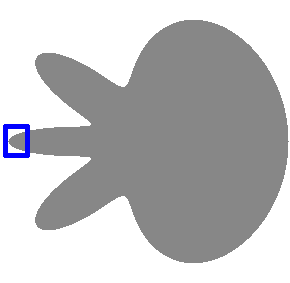
\includegraphics[scale=2.0]{images/local_search/definitions/flower.png}
	}\hspace{40pt}%
	\subfloat[\label{}]{%	
	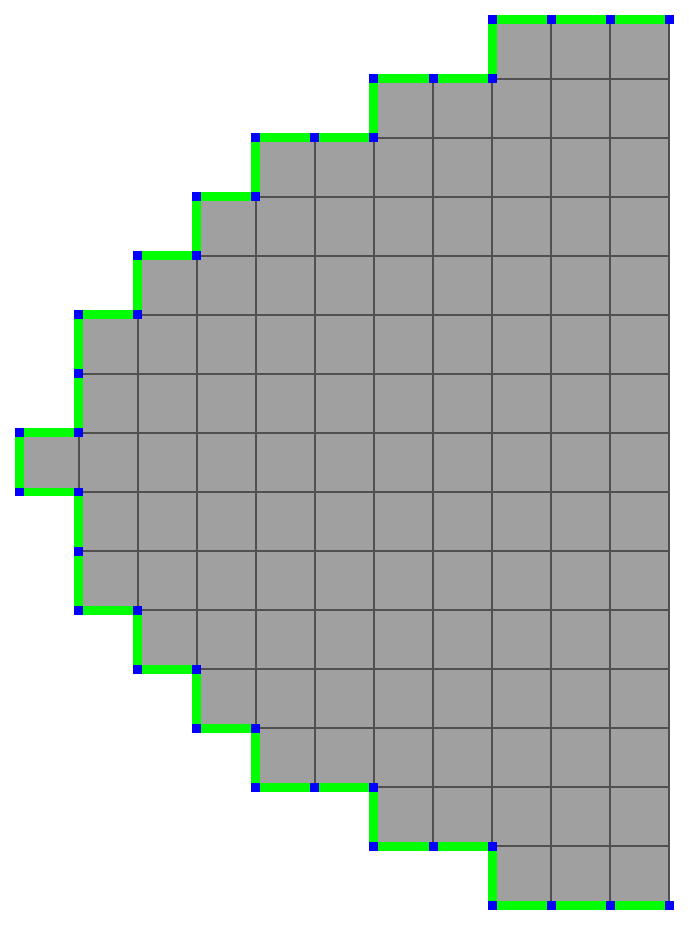
\includegraphics[scale=0.3]{images/local_search/definitions/cellular-grid-illustration.eps}
	}
	\caption{\revision{The flower shape in figure (a) and the cellular-grid model representation in (b) of the rectangle-bounded region. In figure (b), pixels are colored in gray, linels in green and pointels in blue.}}
	\label{fig:cellular-grid-model}
\end{figure}


Let $d_{S}:\Omega \rightarrow \mathbb{R}$ be the \revision{signed} Euclidean distance transformation with respect to shape $S$. The value $d_S(p)$ gives the Euclidean distance between \revision{$p \notin S$ and the closest pixel in $S$. For points $p \in S$, $d_S(p)$ gives the distance between $p$ and the closest pixel not in $S$.}


\begin{definition}[m-Ring Set]
\revision{
Given a digital shape $S\in\Omega$, its signed distance transformation $d_S$ and natural number $m \neq 0$, the {\em $m$-ring set of $S$} is defined as
\begin{align*}
	R_m(S) &:= L_m \cup L_{-m},
\end{align*}
where
\begin{align*}
	L_m(S) &:= \left\{ \quad \begin{array}{cc}
		\left\{ p \in \Omega \; | \; m-1 < d_S(p) \leq m \right\} & , \quad m>0\\
		\left\{ p \in \Omega \; | \; m+1 > d_S(p) \geq m \right\} & , \quad m<0
		\end{array} \right.
\end{align*}}
\end{definition}

Consider the following set of neighbor candidates to $S$:
\begin{align*}
\mathcal{U}(S) = \{ D \; | D \subset R_1(S) \cup S \; \text{and} \; \text{$D$ is connected} \}.
\end{align*}


Such set can be extremely large and its complete exhaustion is prohibitively expensive.  Instead, we are going to use a subset of it.

\begin{definition}[$n$-neighborhood]
\revision{
	Given a digital shape $S \in \Omega$, its $n$-neighborhood $\mathcal{N}_n(S)$ is defined as the set of digital shapes that can be built from $S$ by adding or removing a sequence of $n$ connected pixels in $R_1(S)$.
}
\end{definition}


\begin{figure}[!h]
\center
	\subfloat[\label{}]{%
	\includegraphics[scale=0.03]{images/local_search/definitions/R3.pdf}
	}\hspace{40pt}%
	\subfloat[\label{}]{%
	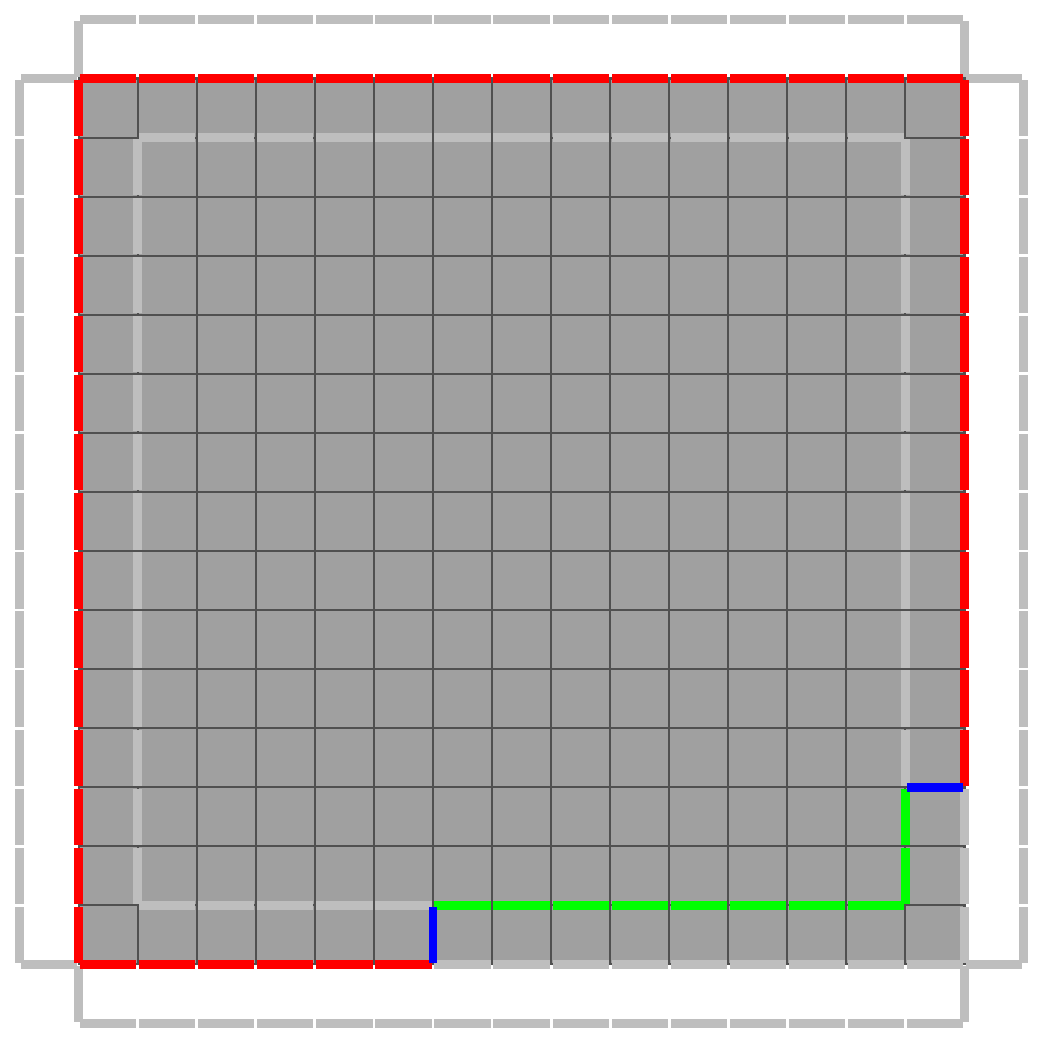
\includegraphics[scale=0.22]{images/local_search/definitions/glued-curve.eps}
	}%	
	\caption{\revision{The blue pixels in figure (a) illustrates a $3$-ring set. In figure (b) we highlight the contour of an element of set $\mathcal{N}_{11}$.}}
\end{figure}

Algorithm~\ref{alg:local-search} describes the local combinatorial process and Figure~\ref{fig:local-comb-square-results} presents the digital curve evolution when executing this algorithm for two different shapes with \revision{$0 \leq n \leq 50$}.


\begin{algorithm}
 \SetKwData{It}{i}
 \SetKwData{MIt}{maxIt}
 \SetKwData{Tol}{tolerance}
 \SetKwData{Delta}{delta}
 \SetKwData{Best}{best} 
 \SetKwInOut{Input}{input}\SetKwInOut{Output}{output}
 
 \Input{A digital set $S$; the neighborhood parameter $n$; the maximum number of iterations \MIt; and a stop condition \Tol}
 \BlankLine
 \Delta $\longleftarrow$ \Tol+1\;
 $i \longleftarrow 0$\;
 \While{ \It $<$ \MIt \bf{and} \Delta $>$ \Tol  }{
  	\For{$ X \in \mathcal{N}_n(S^{(i)}) $}
	{
		\If{ $\hat{E}(X)$ $<$ $\hat{E}(X^\star)$ }
		{
			$X^\star \longleftarrow X$
		}
	}
	\It $\longleftarrow$ \It $+1$\;
	$S^{(i)} \longleftarrow X^\star$\;
	\Delta $\longleftarrow$ $\hat{E}(S^{(i-1)}) - \hat{E}(S^{(i)})$\;	
 }
 \caption{Local combinatorial optimization for \revision{E}lastica minimization.}
 \label{alg:local-search} 
\end{algorithm}

		
\begin{figure}[!h]
	\center
	\begin{tabular}{ccc}
		$h=1.0$ & $h=0.5$ & $h=0.25$\\
		\includegraphics[scale=0.2]{images/local_search/square/h1/summary.eps} & 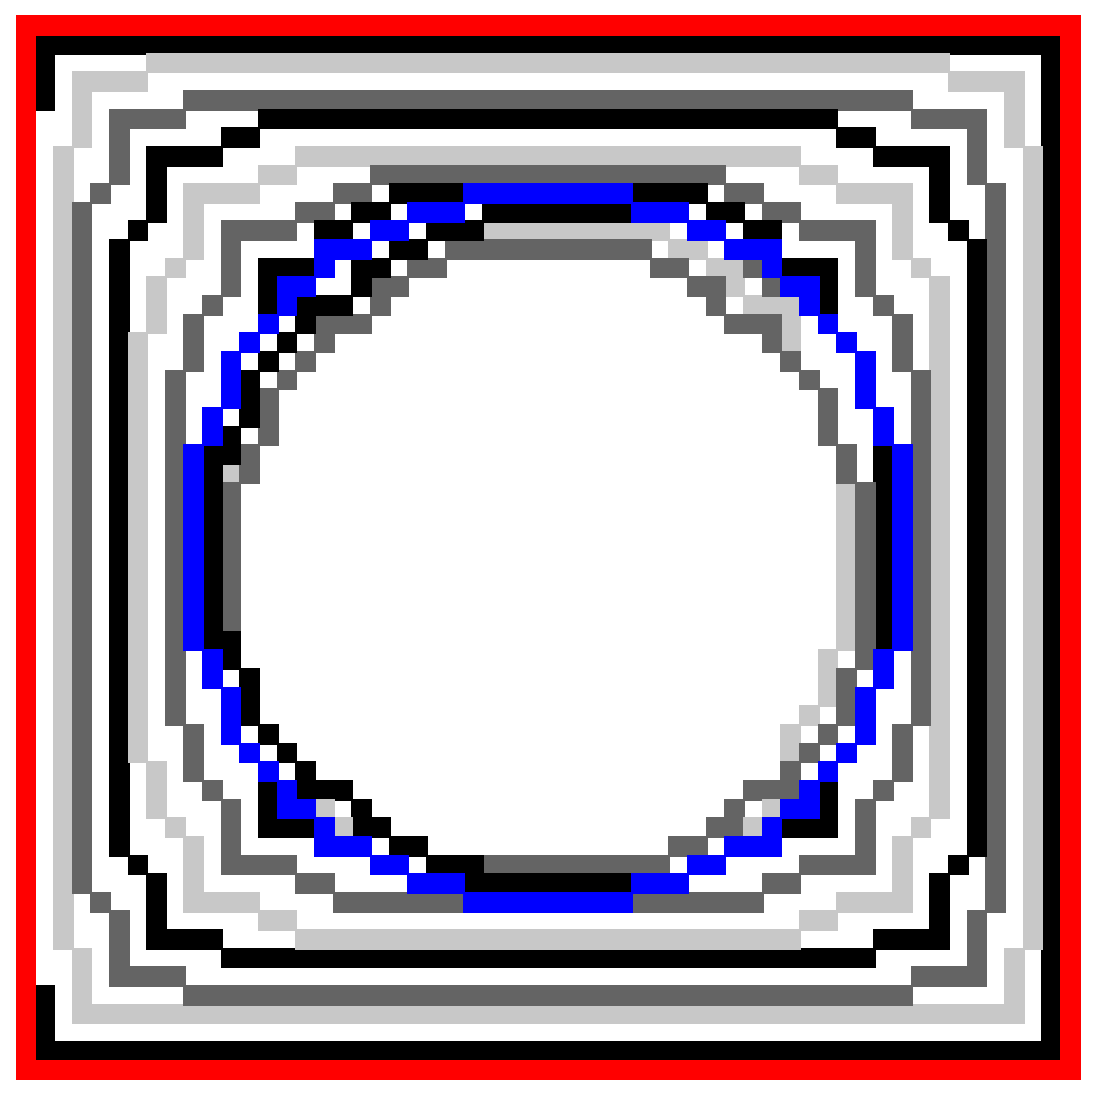
\includegraphics[scale=0.2]{images/local_search/square/h05/summary.eps} & 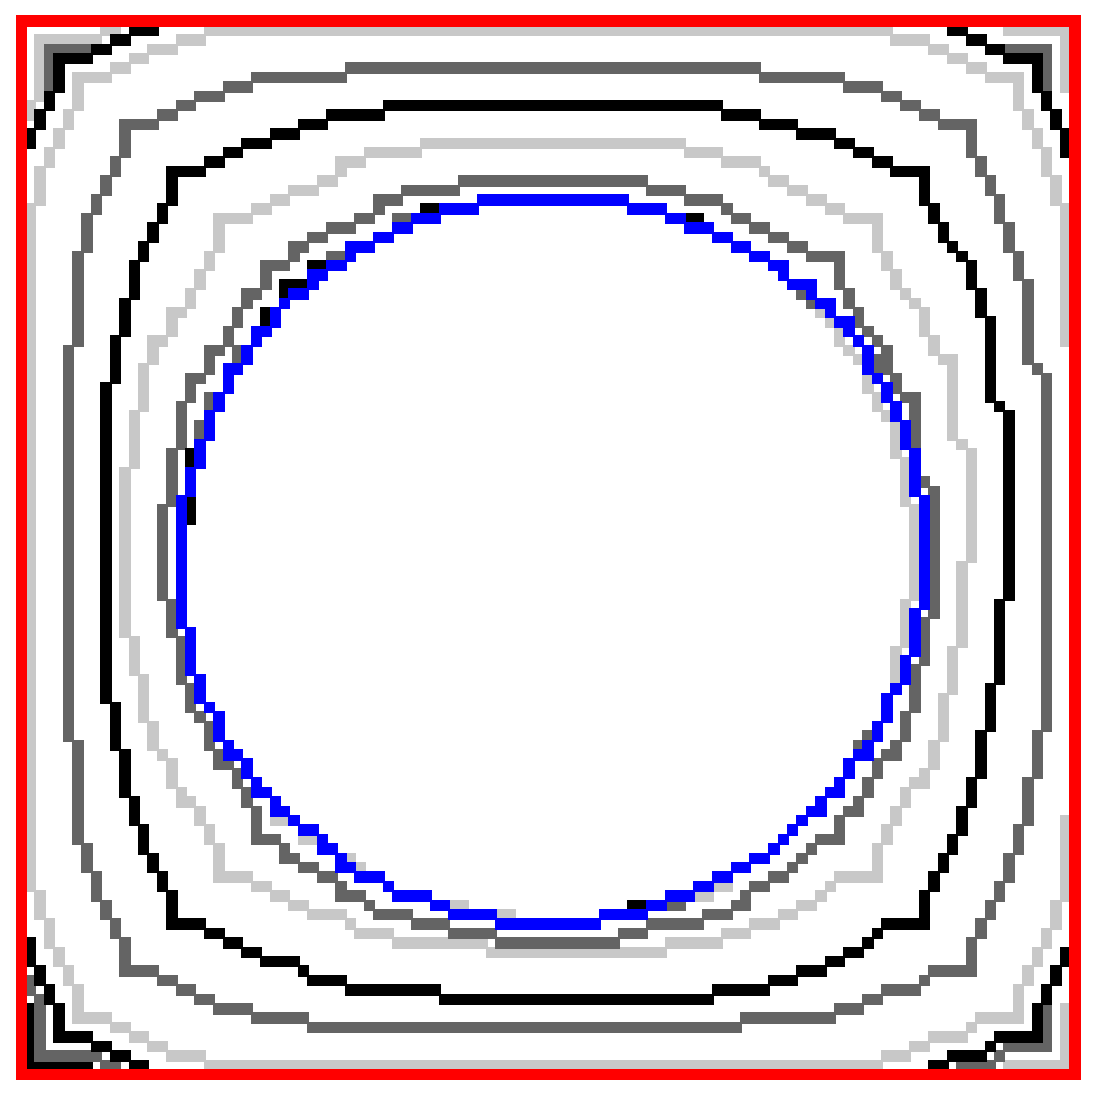
\includegraphics[scale=0.2]{images/local_search/square/h025/summary.eps} \\
		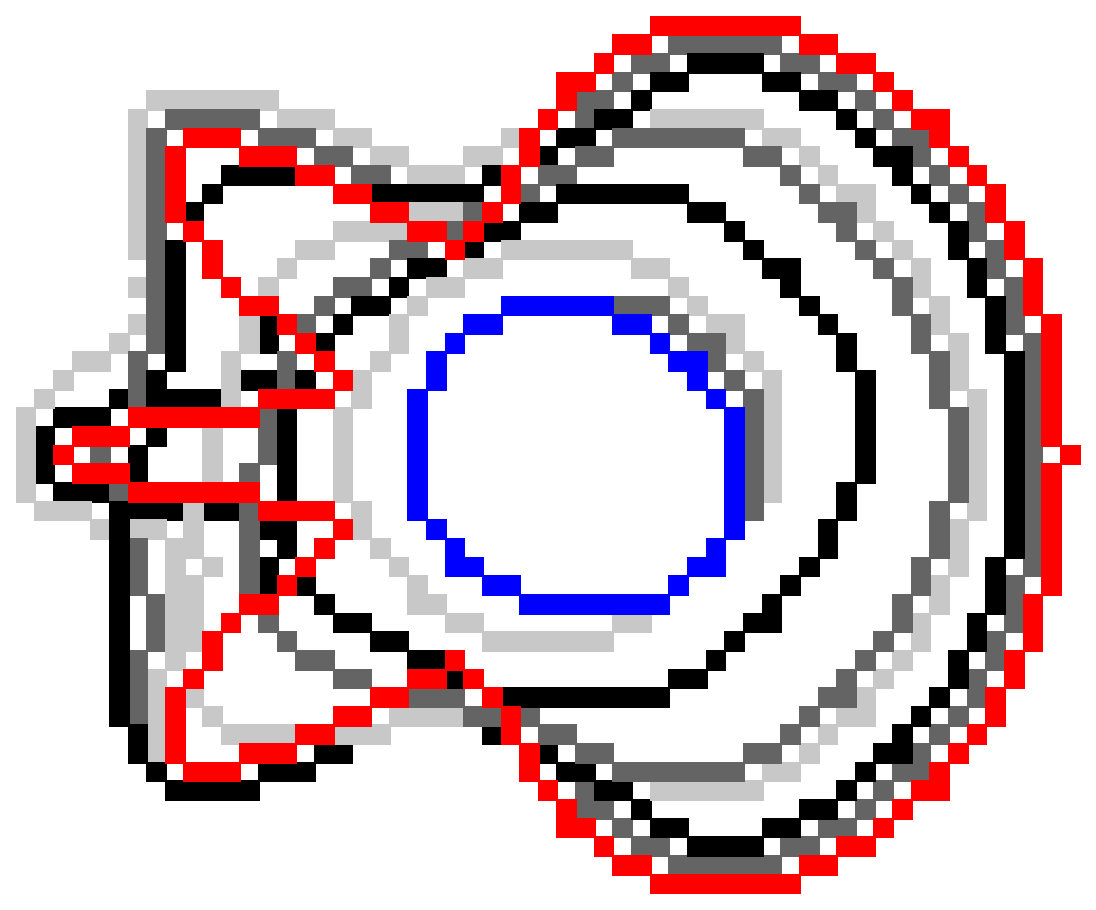
\includegraphics[scale=0.2]{images/local_search/flower/h1/summary.eps} & 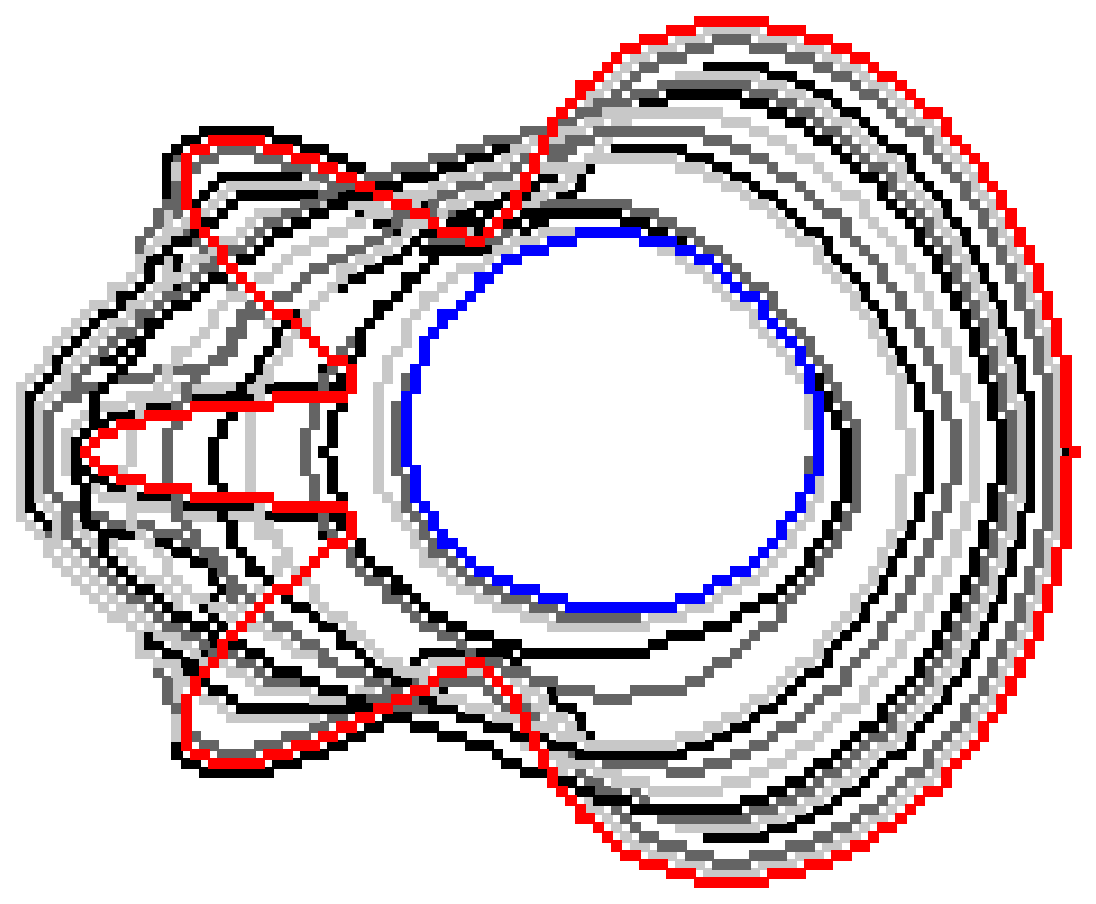
\includegraphics[scale=0.2]{images/local_search/flower/h05/summary.eps} & \includegraphics[scale=0.2]{images/local_search/flower/h025/summary.eps}
	\end{tabular}	
		\caption{\revision{Local combinatorial optimization process results using II estimator with radius $5$ for the square and flower shapes. Shapes are displayed at every $5$ iterations.}}	
		\label{fig:local-comb-square-results}		
\end{figure}


The running time of algorithm \ref{alg:local-search} is summarized in table \ref{tab:summary-local-comb-rtime}. All the
experiments in this paper were executed on a \revision{$32$-core $2.4Ghz$ CPU and the number of pixels in the square and
flower shapes are respectively $841,1641$ for grid step $h=1.0$}. Although its use in practical applications is
limited, we demonstrate that digital estimators are effective in their measurements and the flows evolve as expected. \revision{In particular, the digital elastica energy for the experiments in figure \ref{fig:local-comb-square-results} approaches the global optimum (figure  \ref{fig:plot-elastica-local-search})}. We
observe that it is a complete digital approach, and we do not suffer from discretization and rounding problems, a common
issue in continuous models.  Furthermore, we have checked that this approach works indifferently with Integral Invariant
curvature estimator and Maximal Digital Circular Arc curvature estimator. So the convergence of the digital curvature
estimator seems to be the cornerstone to get a digital curve behaving like a continuous Elastica.  In the next section,
we explore a more efficient approach.

\begin{figure}
	\center
	\captionsetup{type=table}	
	\revision{
	\begin{tabular}{|c|c|c|}
	\hline
	& Square & Flower \\
	\hline
	$h=1.0$ & 4s & 124s \\
	\hline
	$h=0.5$ & 77s & 1924s\\
	\hline
	$h=0.25$ & 1886s & 28445s\\
	\hline
	\end{tabular}
	}
	\caption{Running times for the local combinatorial optimization algorithm with $0 \leq n \leq 50$. Thirty two threads were used.}
	\label{tab:summary-local-comb-rtime}
\end{figure}


\begin{figure}[!h]
\center
\subfloat[\label{}]{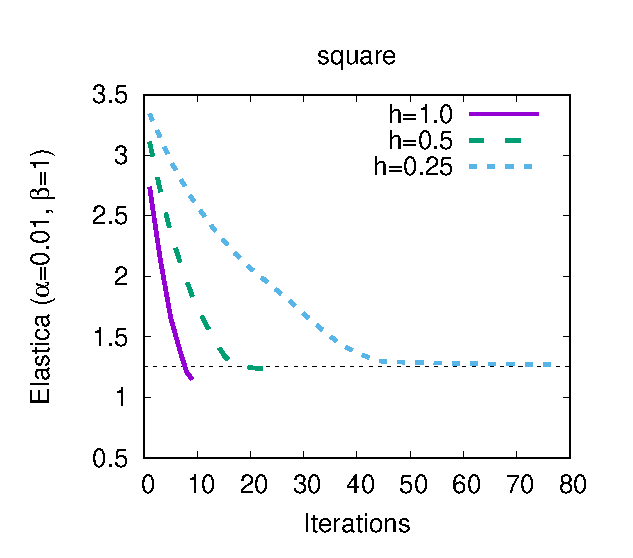
\includegraphics[scale=0.6]{images/local_search/square.eps}}
\subfloat[\label{}]{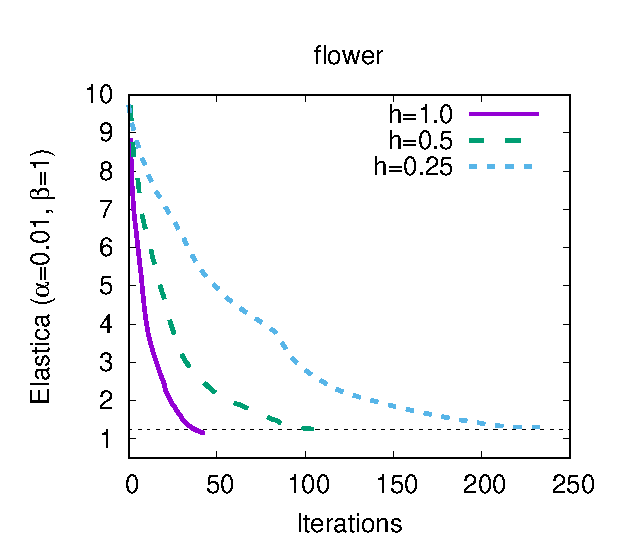
\includegraphics[scale=0.6]{images/local_search/flower.eps}}
\caption{Digital elastica computation along iterations of algorithm \ref{alg:local-search}. \revision{The final shape has energy value closer to the optimal value $2\pi/5$ (thin horizontal dashed line)}.}
\label{fig:plot-elastica-local-search}
\end{figure}

\section{Digital Curvature Flow}

\revision{
Given a digital shape $S \subset \Omega \subset \mathbb{Z}^2$, the goal is to compute a flow $S^{(i)}$ where $S^{(i+1)}$ has lower digital elastica than $S^{(i)}$.}

\revision{We observe that the integral invariant estimator \eqref{eq:curvature_approximation} is originally designed to be evaluated on the digital boundary of the shape, which is the unknown of our problem. Injecting contour information leads to a third-order model, which we prefer to avoid. Instead, we are going to exploit the II estimator definition to compute a flow that evolves proportionally to the squared curvature of the current shape.}

\subsection{Discrete variational model for discrete curve evolution}

\revision{We assume an ordering in $\Omega$, i.e., there exists a bijective function $\omega : \Omega \rightarrow \{1 \cdots |\Omega| \}$. Moreover, we associate to any subset $P \subset \Omega$ the set of binary variables $X(P)$ defined as}

\begin{align*}
	\revision{X(P) := \left\{ x_{\omega(p)} \in \{0,1\} \; | \; p \in P \right\}.}
\end{align*}

In order to guarantee connectivity, we limit the optimization region to a subset of $\Omega$, namely the inner pixel boundary of  $S^{(i)}$. We also use the notation $| S |$ to denote the cardinal of a digital set $S$.

\begin{definition}[Inner pixel boundary]

Given a digital shape $S$ embedded in a domain $\Omega$, we define its inner pixel boundary set \revision{$I(S)$} as
\begin{align*}
	\revision{I(S)} := \left\{ \: p \; | \; p \in S, |\mathcal{N}_4(x) \cap S|<4 \: \right\},
\end{align*}
where $\mathcal{N}_4(p)$ denotes the $4$-adjacent neighbor set of $p$ (without $p$).
\end{definition}



\revision{To simplify notation, the inner pixel boundary of $S^{(i)}$ is simply denoted $I^{(i)}$. At each iteration, the set $X^{(i)}$ of optimization variables is defined as}

\begin{align*}
\revision{
	X^{(i)} := X(I^{(i)}).
}
\end{align*}


In other words, each flow iteration decides which pixels in the inner boundary are to be removed from \revision{$S^{(i)}$} and which are to be kept in \revision{$S^{(i)}$}. We recall the definition of our digital curvature estimator:
\begin{align}
	\hat{\kappa}^2(p) &= c_1\Big( c_2 - | B_r(p) \cap S^{\revision{(i)}} | \Big)^2, 
	\label{eq:curvature-estimator-pixels}
\end{align}
where $c_1=3/r^6$ and $c_2=\pi r^2/2$. 

\revision{The following sets are important in the expansion of $\eqref{eq:curvature-estimator-pixels}$.}

\revision{
\begin{align*}
	F_r^{(i)}(p) &:= \big( S^{(i)} \setminus I^{(i)} \big) \cap B_r(p)\\
	I_r^{(i)}(p) &:= I^{(i)} \cap B_r(p) \\
	X_r^{(i)}(p) &:= X\big( I_r^{(i)}(p) \big).
\end{align*}
}

Expanding \eqref{eq:curvature-estimator-pixels}, we get 

\begin{align*}
  \hat{\kappa}^2(p) &= c_1\Big( c_2 - |F_{r}^{(i)}(p)| - \sum_{x_j \in X_r^{(i)}(p)} {x_j} \Big)^2 \\
   &= c_1 \Big( C + 2\left( |F_{r}^{(i)}(p)| - c_2 \right) \hspace{-2mm}\sum_{x_j \in X_{r}^{(i)}(p)}\hspace{-2mm}{x_j} + \hspace{-2mm}\sum_{x_j \in X_{r}^{(i)}(p)}\hspace{-2mm}{x_j^2} + \hspace{-2mm}\sum_{ \substack{x_j,x_k \in X_{r}^{(i)}(p) \\ j<k} }\hspace{-2mm}{2x_jx_k}  \Big),
\end{align*}
where $C=c_2^2 - 2c_2 \cdot |F_{r}^{(i)}(p)| + |F_{r}^{(i)}(p)|^2$ is a constant. By ignoring constants and multiplication factors and using
the binary character of the variables, we define the following family
of energies for given parameters $\alpha,\beta, \gamma \geq 0$.
\begin{align}
  E_m(X^{\revision{(i)}},S^{\revision{(i)}}) =& \sum_{x \in X^{\revision{(i)}}}{\alpha s(x)} + \nonumber \\ 
  & \sum_{ \substack{p \in \\ R_m(S^{\revision{(i)}})}}{ \revision{2c_1} \beta  \Big( { (1/2+ |F_{r}^{(i)}(p)|-c_2) \cdot \sum_{ \substack{ x_j \in \\ X_{r}^{(i)}(p)}}{x_j} } + \sum_{ \substack{j<k, \\ x_j,x_k \in \\ X_{r}^{(i)}(p) } }{x_jx_k} \Big) } + \nonumber \\
  & \sum_{x \in X^{\revision{(i)}}}{\gamma g(S^{\revision{(i)}},x)},
  \label{eq:energy-family}
\end{align}
where $g(S,x)$ denotes a \revision{data term (e.g., distance to initial shape $S$ or fidelity to data)} and $s(x)$ denotes a length penalization term. Each choice of $m$ generates a different flow, which is generally described in the Digital Curve Evolution (DCE) algorithm \ref{alg:evolution-model}.


\begin{figure}
\begin{minipage}{0.5\textwidth}
\center
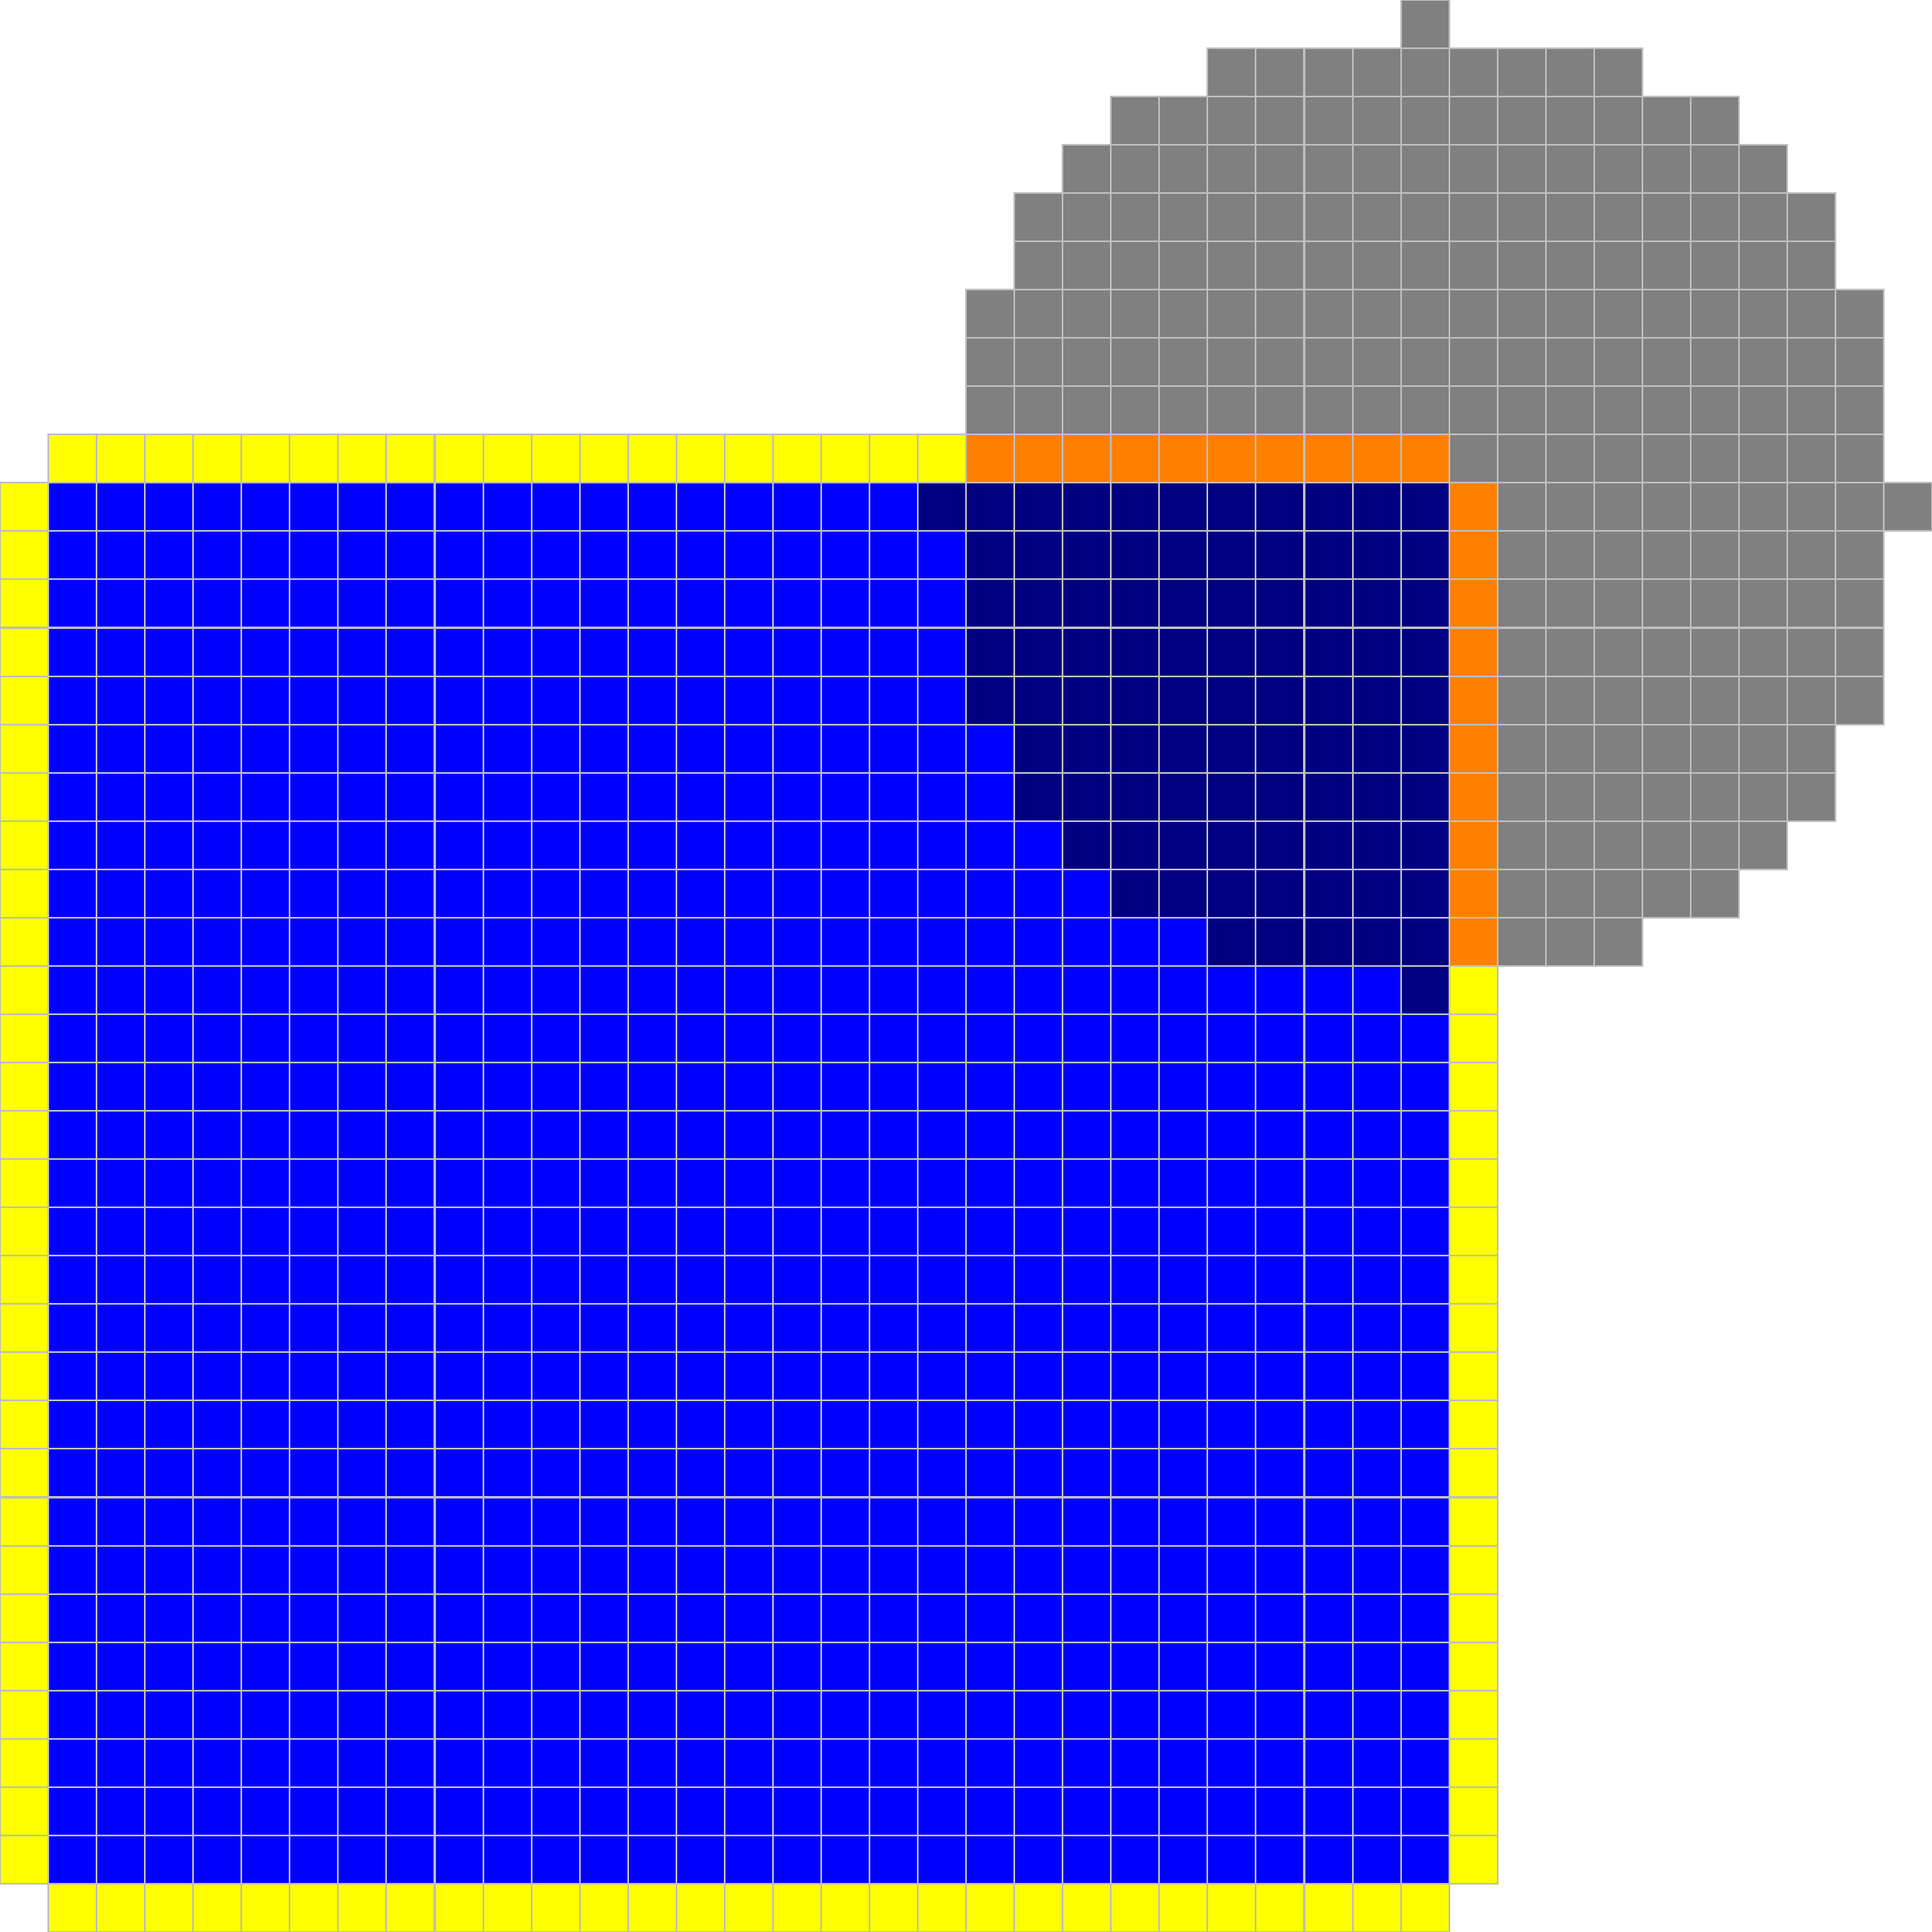
\includegraphics[scale=0.1]{images/flow/contour-information/before-opt.pdf}
\label{fig:contour-info-1}
\end{minipage}%
\begin{minipage}{0.5\textwidth}
\center
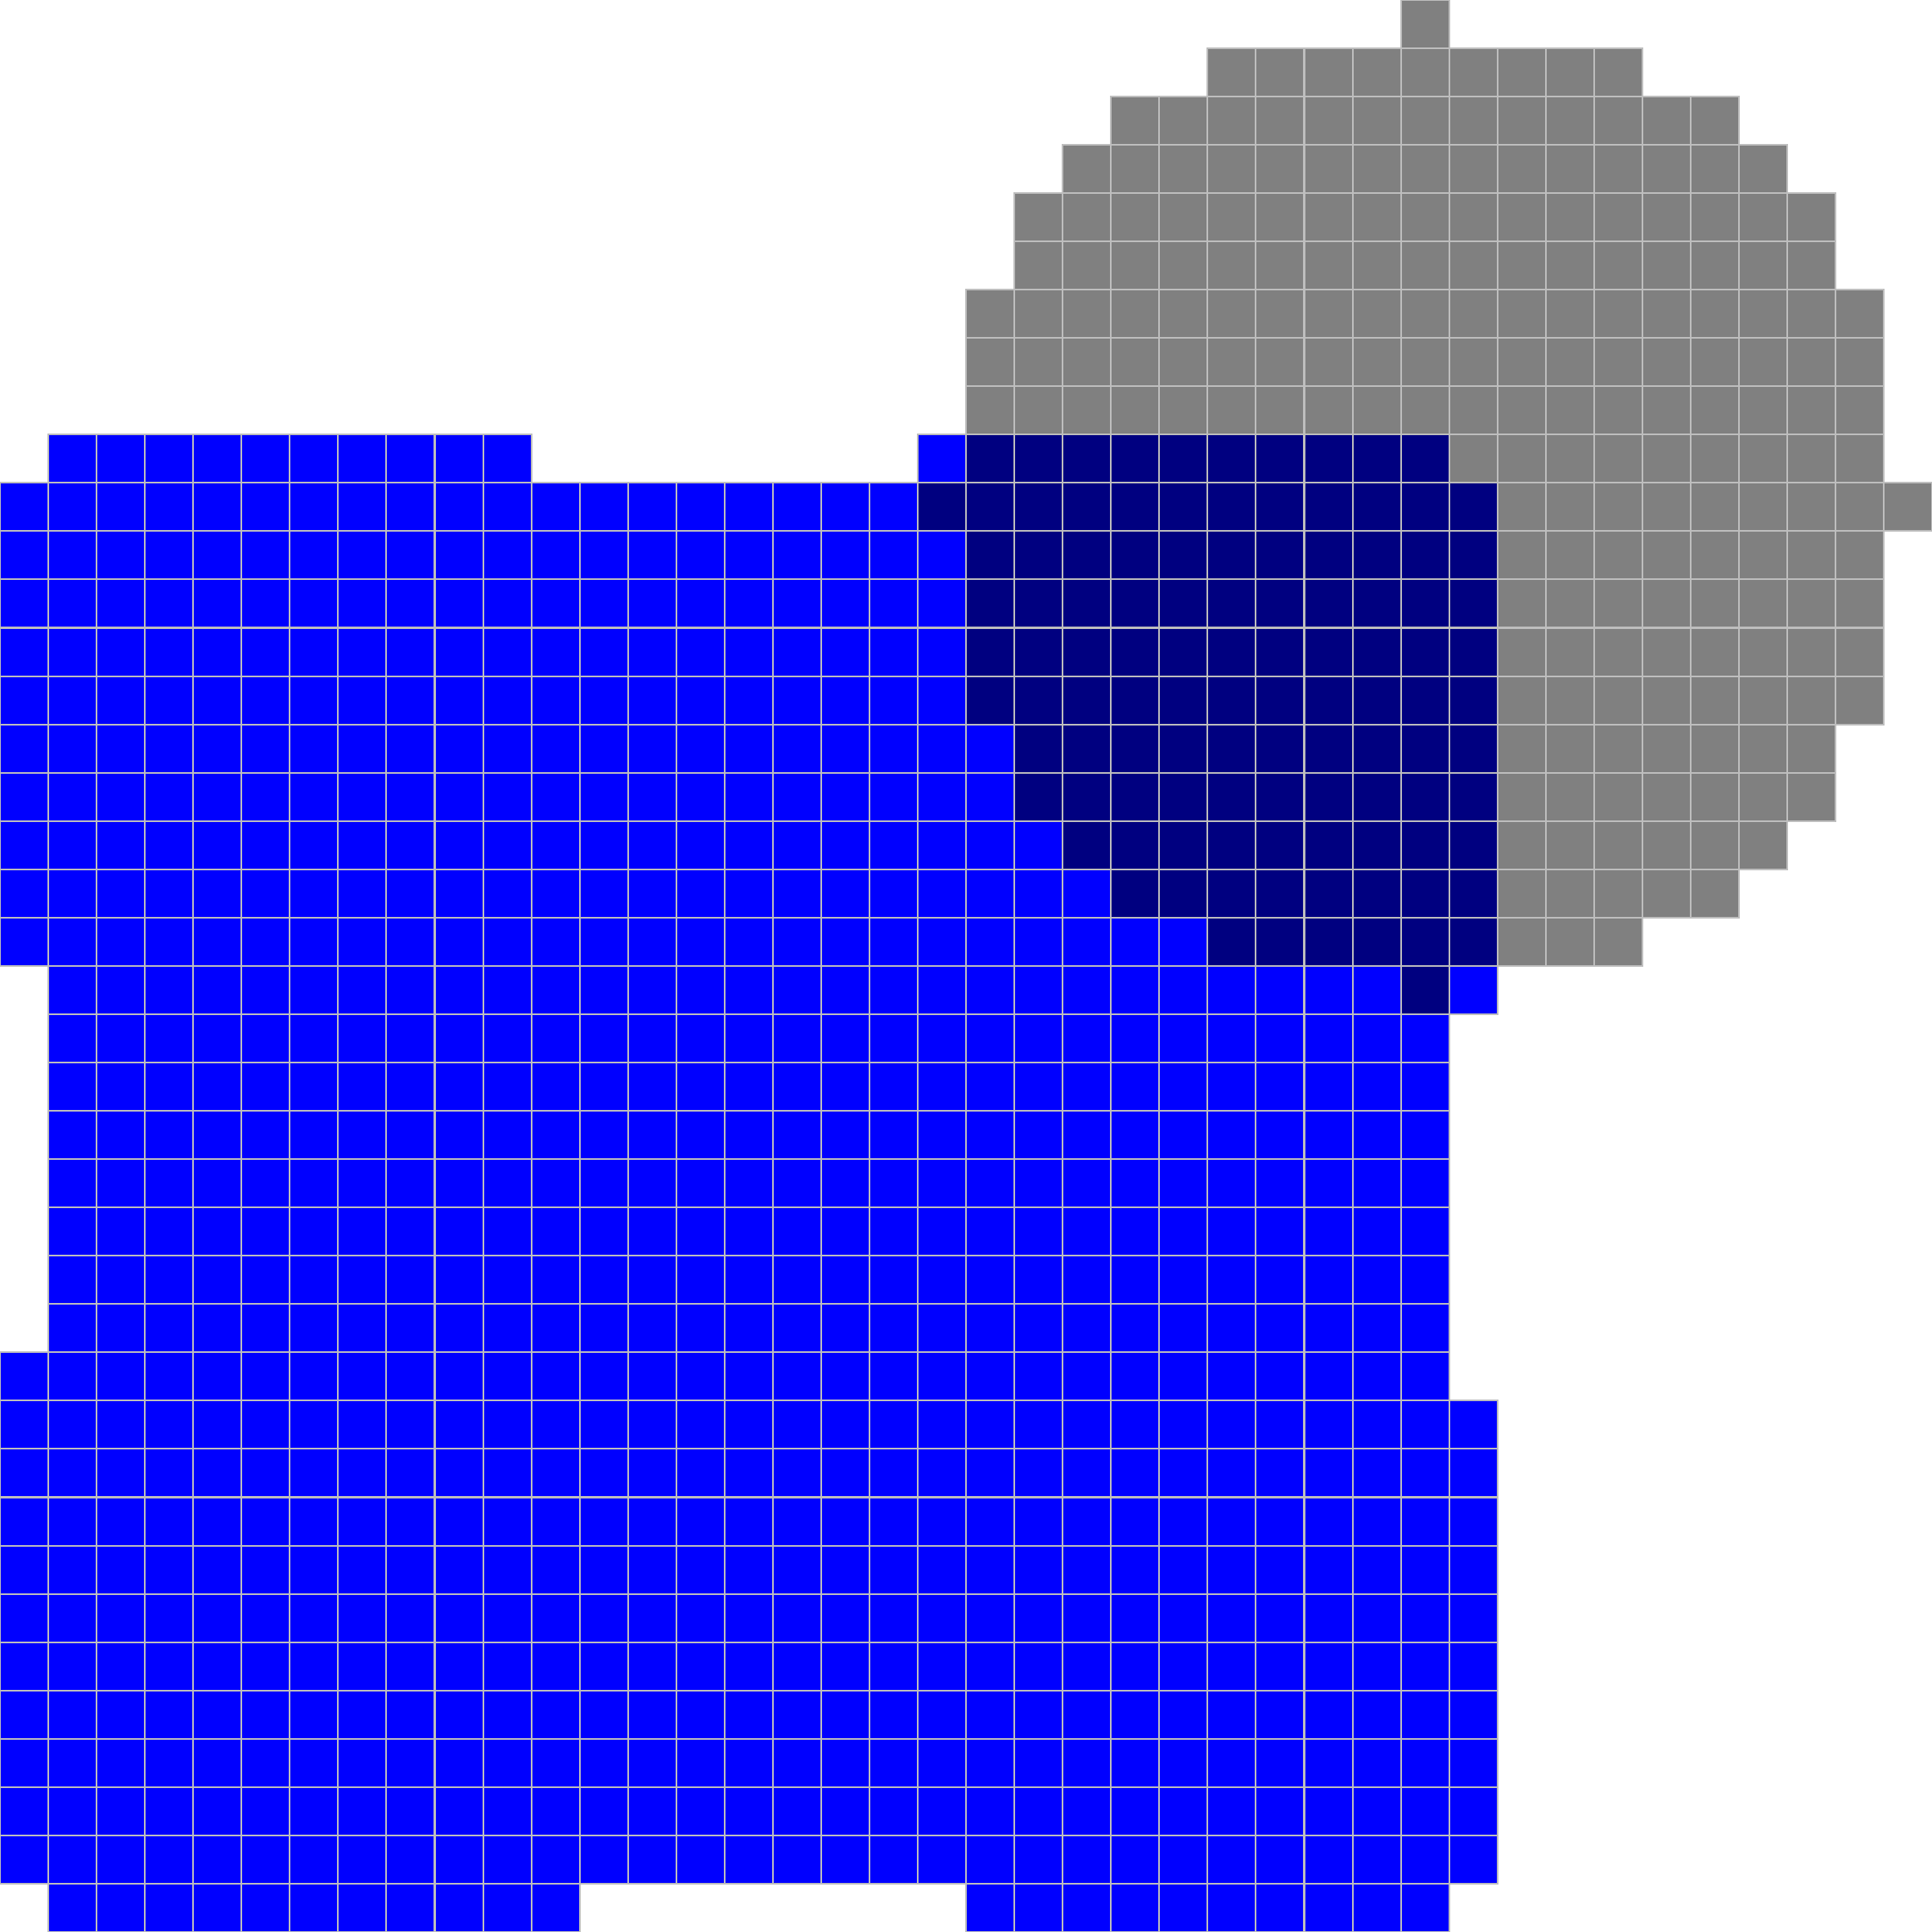
\includegraphics[scale=0.1]{images/flow/contour-information/after-opt.pdf}
\label{fig:contour-info-2}
\end{minipage}%
\caption{ \revision{Directly using the optimization result of \eqref{eq:energy-family} doesn't decrease squared curvature because contour information is not present in the energy.}}
\label{fig:contour-info}
\end{figure}

\begin{algorithm}
 \SetKwData{It}{i}
 \SetKwData{MIt}{maxIt}
 \SetKwData{Delta}{delta}
 \SetKwInOut{Input}{input}\SetKwInOut{Output}{output}
 \SetKwComment{comment}{//}{}
 
 \Input{A digital set $S$; The ring number $m$; Length($\alpha$), curvature($\beta$) and \revision{data}($\gamma$) coefficients; the maximum number of iterations \MIt;}
 \BlankLine
 $S^{(0)} \longleftarrow S$\;
 $i \longleftarrow 1$\;
 \While{ \It $<$ \MIt  }{ 	
	\comment{Expansion mode}
	\If{ \It is odd }{	 
	 	$X^{(i)} \longleftarrow \argmin_X E_m(X,\overline{S^{(i-1)}})$\;
 		$\revision{S^{(i)} \longleftarrow \overline{ F^{(i-1)}_{\overline{S}} + \overline{X^{(i)}}}}$\;
 	}
	\comment{Shrinking mode} 	
 	\Else{	
	 	$X^{(i)} \longleftarrow \argmin_X E_m(X,S^{(i-1)})$\; 	
 		$S^{(i)} \longleftarrow F^{(i-1)}_{S} + \overline{X^{(i)}}$\;
 	}
 	
	\It $\longleftarrow$ \It $+1$\;
	
 }
 \caption{Digital curvature evolution algorithm (DCE).}
 \label{alg:evolution-model}  
\end{algorithm}

\revision{
We emphasize that the minimization of \eqref{eq:energy-family} for $S^{(i)}$ is not sufficient to derive the next shape $S^{(i+1)}$ because contour information is not included in the model (see figure \ref{fig:contour-info})}. Recall that the integral invariant estimator approaches curvature by computing the difference between half of the area
of a chosen ball and the area of the intersection of this ball with the shape.  In particular, regions of positive
curvature have fewer pixels in their intersection set than on its complement w.r.t the estimation ball. This implies
that variables in such regions are labeled with 1, as the unbalance grows otherwise. We attenuate curvature if we shift
the center of the estimation ball towards the interior of the shape, which means removing the 1-labeled pixels. That is
why we take the complement of the optimization solution.

The same reasoning applies for non-convex parts. Indeed, concave regions are convex in the shape complement. In the
expansion mode we apply the same reasoning on the image complement, and by doing this we are able to handle
concavities. It is called expansion mode because the optimization region, in this case, is the outer pixel boundary of
the original shape. Table~\ref{tab:flow-summary} sums up these arguments.



Length and \revision{data} terms should be properly defined in order to comply with the complement step of the DCE
algorithm. The length penalization is defined as
\begin{align}
  s(x)=\sum_{x_j \in \mathcal{N}_4(x)}{ t(x_j) }, \quad \text{where } t(x_j) = \left\{\begin{array}{ll}
  (x-x_j)^2, & \text{if } x_j \in X_{r}^{(i)}\\
  (x-0), & \text{if } x_j \in F_{r}^{(i)}\\
  (x-1), & \text{otherwise }
  \end{array}\right.
  \label{eq:length-penalization}
\end{align}
	
We do not use \revision{data} terms in this section, thus we postpone the definition of such terms until later in this
article, with the description of how DCE can be used in an image segmentation framework.



\begin{table}
  \center
  \setlength{\extrarowheight}{0.5em}
  \begin{tabular}{|c|c|c|c|} \hline
    shrink mode &    $\kappa \gg 0$ & $\kappa \geq 0$ &  $\kappa < 0$ \\ \hline
    $X$ & $x_k=1$ & $x_k \in \{0,1\}$ & $x_k=0$ \\ \hline
    $S^{(i+1)} \leftarrow S^{(i)} \setminus X$ & eroded & prob. eroded & unchanged  \\ \hline \hline
    expansion mode &    $\bar{\kappa} \gg 0$ & $\bar{\kappa} \geq 0$ & $\bar{\kappa} < 0$ \\ \hline
    $\bar{X}$ & $\bar{x}_k=1$ & $\bar{x}_k \in \{0,1\}$ & $\bar{x}_k=0$ \\ \hline
    $S^{(i+1)} \leftarrow \overline{\bar{S}^{(i)} \setminus \bar{X}}$ & dilated & prob. dilated & unchanged \\ \hline 
  \end{tabular}
  
  \caption{  Since the curvature is negated when reversing the curve (i.e. $\bar{\kappa}=-\kappa$), this process can only shrink  convex parts in shrink mode and expand concave parts in expansion mode.}
   \label{tab:flow-summary}	  

\end{table}


In figure \ref{fig:m1-square-flow} we see some results for the DCE algorithm with $m=1$. We observe a global evolution
towards rounder shapes, but with several artifacts. We minimize the effects of a jaggy boundary by setting $\alpha >
0$. Nonetheless, a \revision{higher radius of the estimation ball} creates unstable shapes. In fact, the estimator is very sensitive in
regions of low squared curvature, and it is precisely in those regions that spurious pixels are created.


\begin{figure}[!h]
\center
\begin{minipage}[b]{0.33\textwidth}
	\subfloat[$r=3, \alpha=0$\label{}]{%
	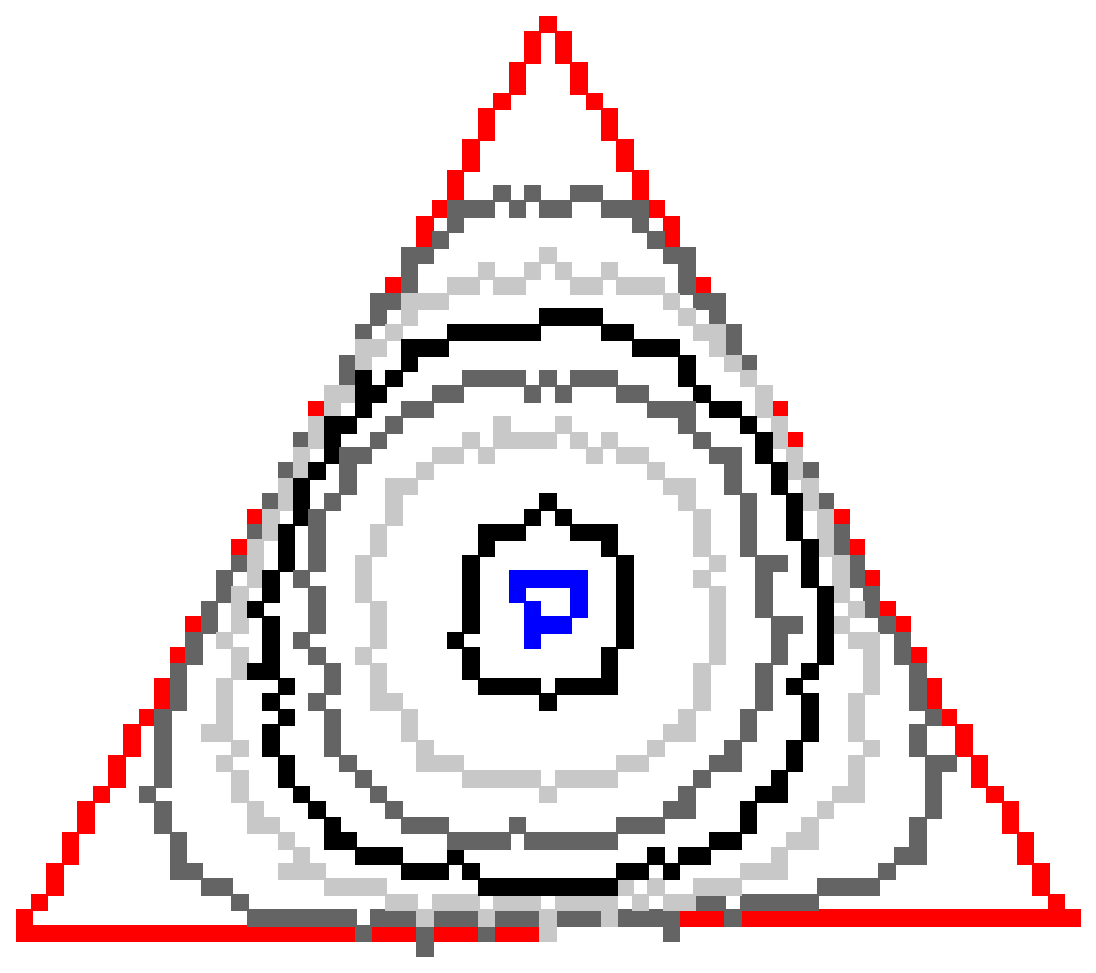
\includegraphics[scale=0.2]{images/flow/length-radius-effect/triangle-r3-nolength/summary_flow.eps}
	}%
\end{minipage}%
\begin{minipage}[b]{0.33\textwidth}
	\subfloat[$r=3, \alpha=0.15$\label{}]{%
	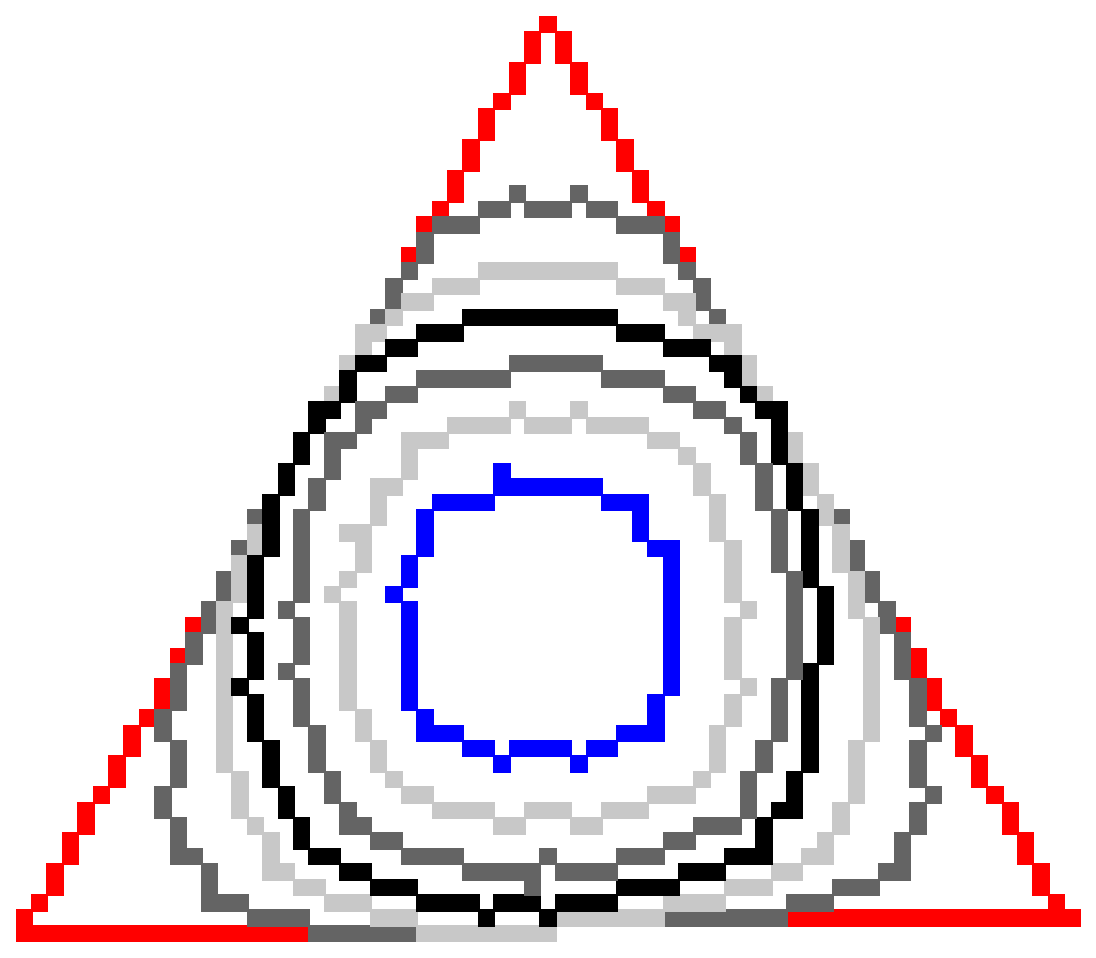
\includegraphics[scale=0.2]{images/flow/length-radius-effect/triangle-r3-length0.15/summary_flow.eps}
	}%
\end{minipage}%
\begin{minipage}[b]{0.33\textwidth}
	\subfloat[$r=5, \alpha=0.15$\label{}]{%
	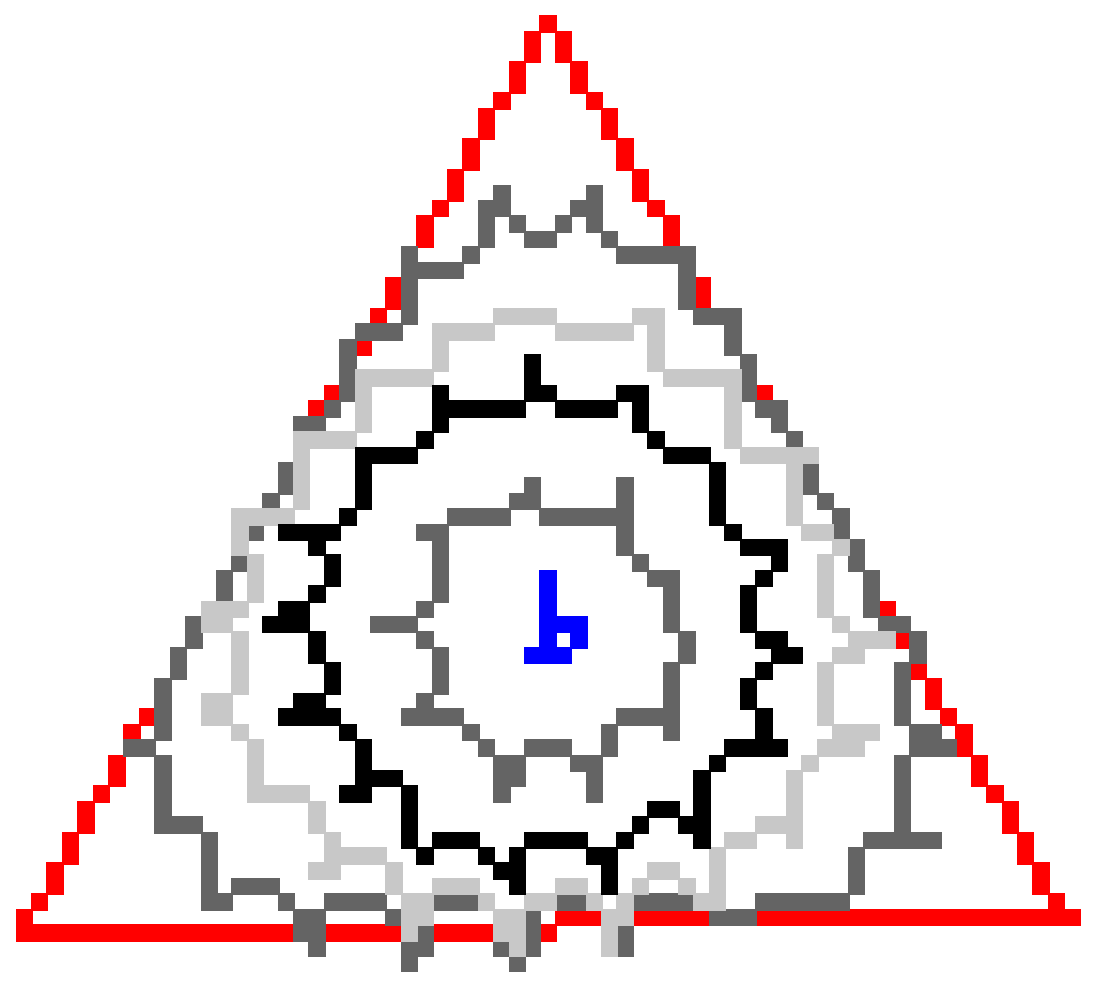
\includegraphics[scale=0.2]{images/flow/length-radius-effect/triangle-r5/summary_flow.eps}
	}%
\end{minipage}%
\caption{The algorithm is very sensitive to the little variations of the estimator, which are particularly important in regions of low squared curvature. Artifacts are somewhat reduced with a length penalization but increases if we use a higher ball radius. }
\label{fig:m1-square-flow}
\end{figure}


\subsection{A more stable model.}
In the previous section we noticed that the algorithm produces shapes with many artifacts due to the small uncertainties
of the estimator along regions of low squared curvature. We argue that, \revision{by} evaluating the estimation ball along outer
ring sets we avoid those sensitive areas by focusing the optimization process only on regions with highest squared
curvature value.


\begin{figure}[!h]
\center
\center
\begin{minipage}[b]{0.33\textwidth}
	\subfloat[$r=5, m=1$\label{}]{%
	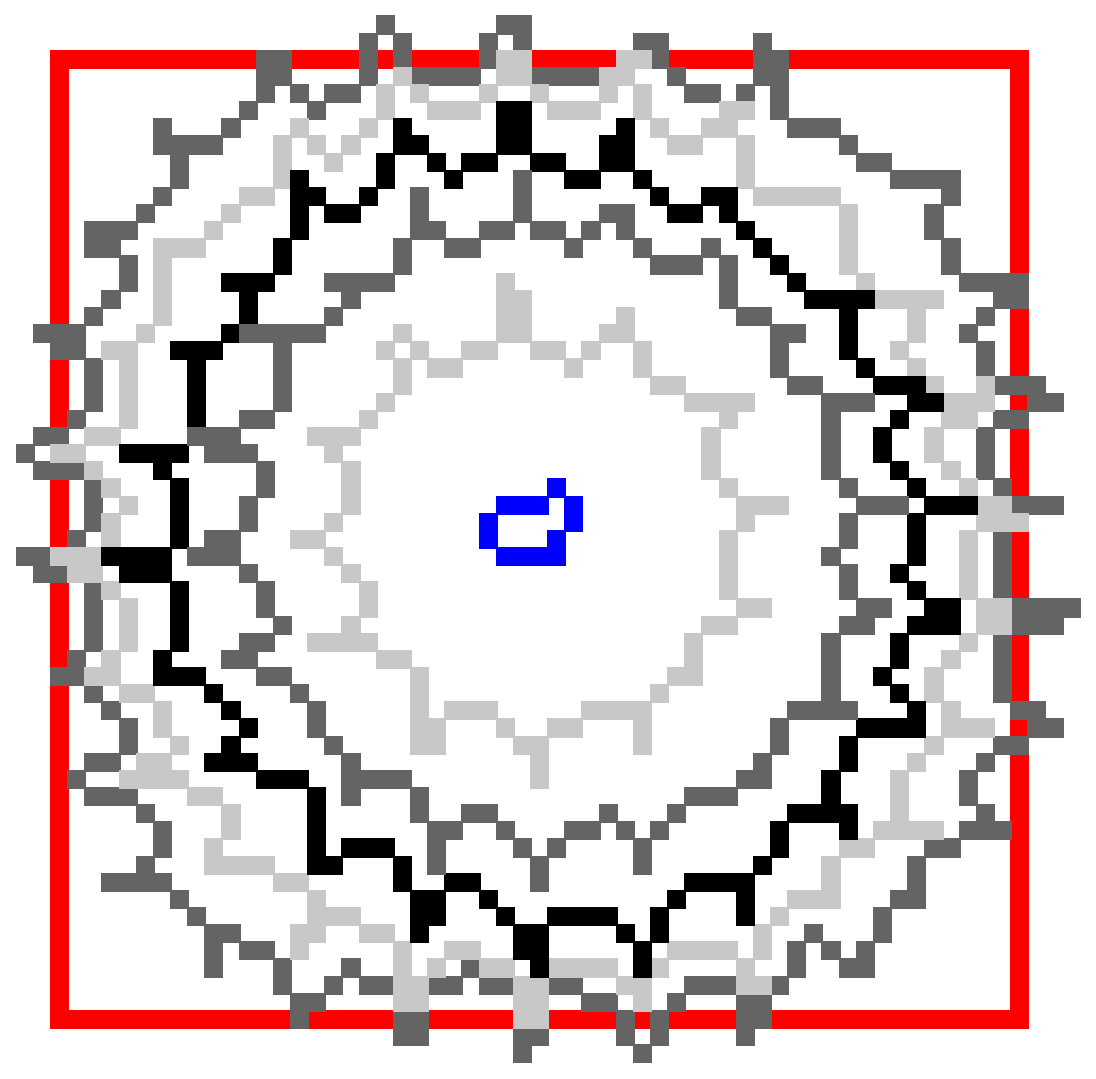
\includegraphics[scale=0.2]{images/flow/farther-rings/square-r5-l1/summary_flow.eps}
	}%
\end{minipage}%
\begin{minipage}[b]{0.33\textwidth}
	\subfloat[$r=5, m=3$\label{}]{%
	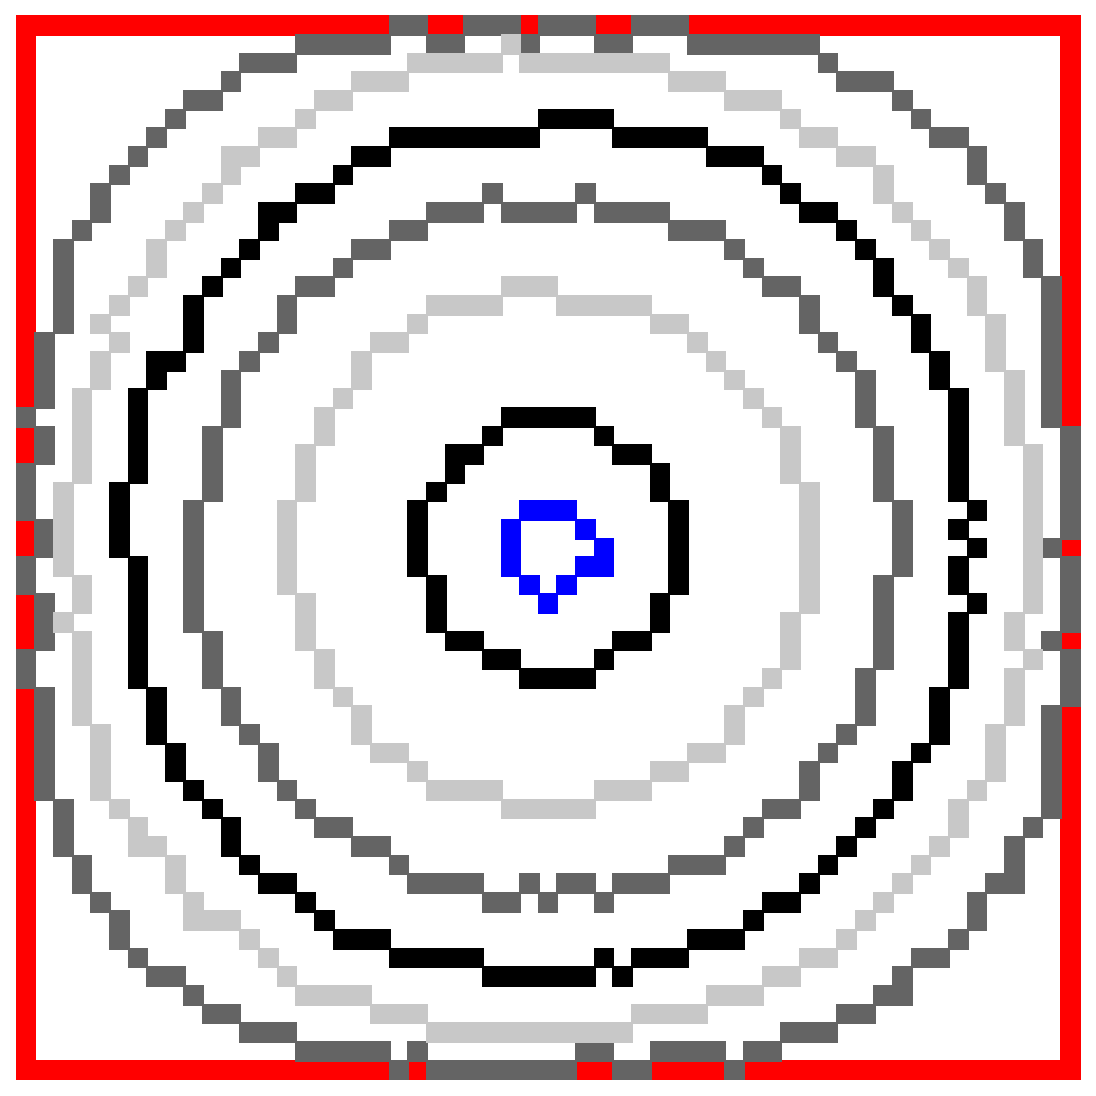
\includegraphics[scale=0.2]{images/flow/farther-rings/square-r5-l3/summary_flow.eps}
	}%
\end{minipage}%
\begin{minipage}[b]{0.33\textwidth}
	\subfloat[\revision{$r=5, m=5$}\label{}]{%
	\includegraphics[scale=0.2]{images/flow/farther-rings/square-r5-l5/summary_flow.eps}
	}%
\end{minipage}%
\caption{By positioning the estimation ball on farther rings, we minimize artifacts creation. \label{fig:mx-square-flow}}
\end{figure}

{In our experiments, the best results are obtained by executing DCE algorithm with $m$ equal to $r$, where $r$ is
  the estimation ball radius (see figure \ref{fig:mx-square-flow}). We observe that digital elastica may increase after some
  iterations if chosen radius is too large, as in the case of the triangle in figure \ref{fig:mx-flow-gs-radius-effect}
  in which the flow converges to a single point. We conjecture that an appropriated value for the radius should be given
  by the shape reach.  The produced flow has no difficulties in handling changes on topology, and it presents different
  speeds for regions with low and high curvature values, as illustrated in figure
  \ref{fig:mx-speed-variation-hole-filling}.

\begin{figure}[hp!]
\center				
		\setcounter{subfigure}{-3}
		\subfloat[$r=3,h=0.5$]{%
		\subfloat{%
		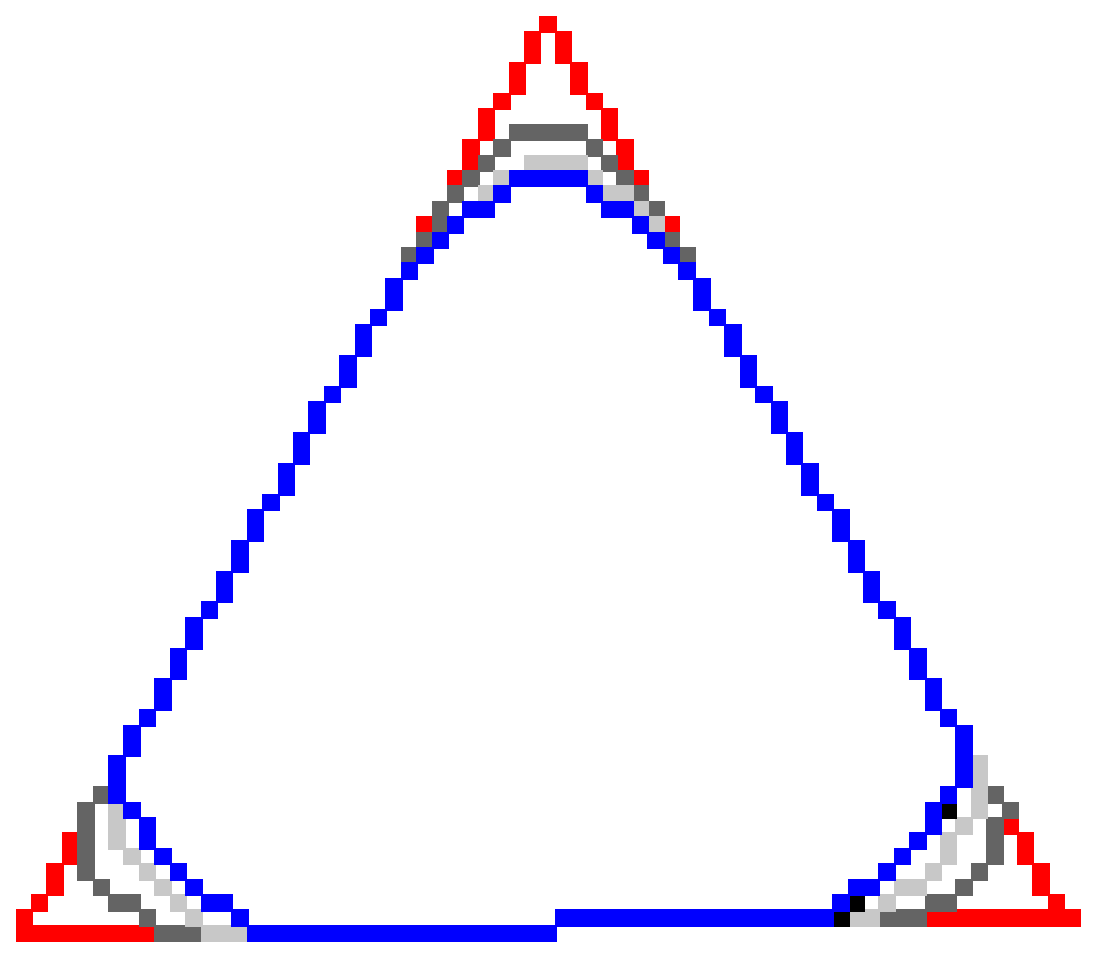
\includegraphics[scale=0.2]{images/flow/grid-radius-effect/triangle/r3-h0.5/summary_flow.eps}
		}%
		\hspace{15pt}
		\subfloat{%
		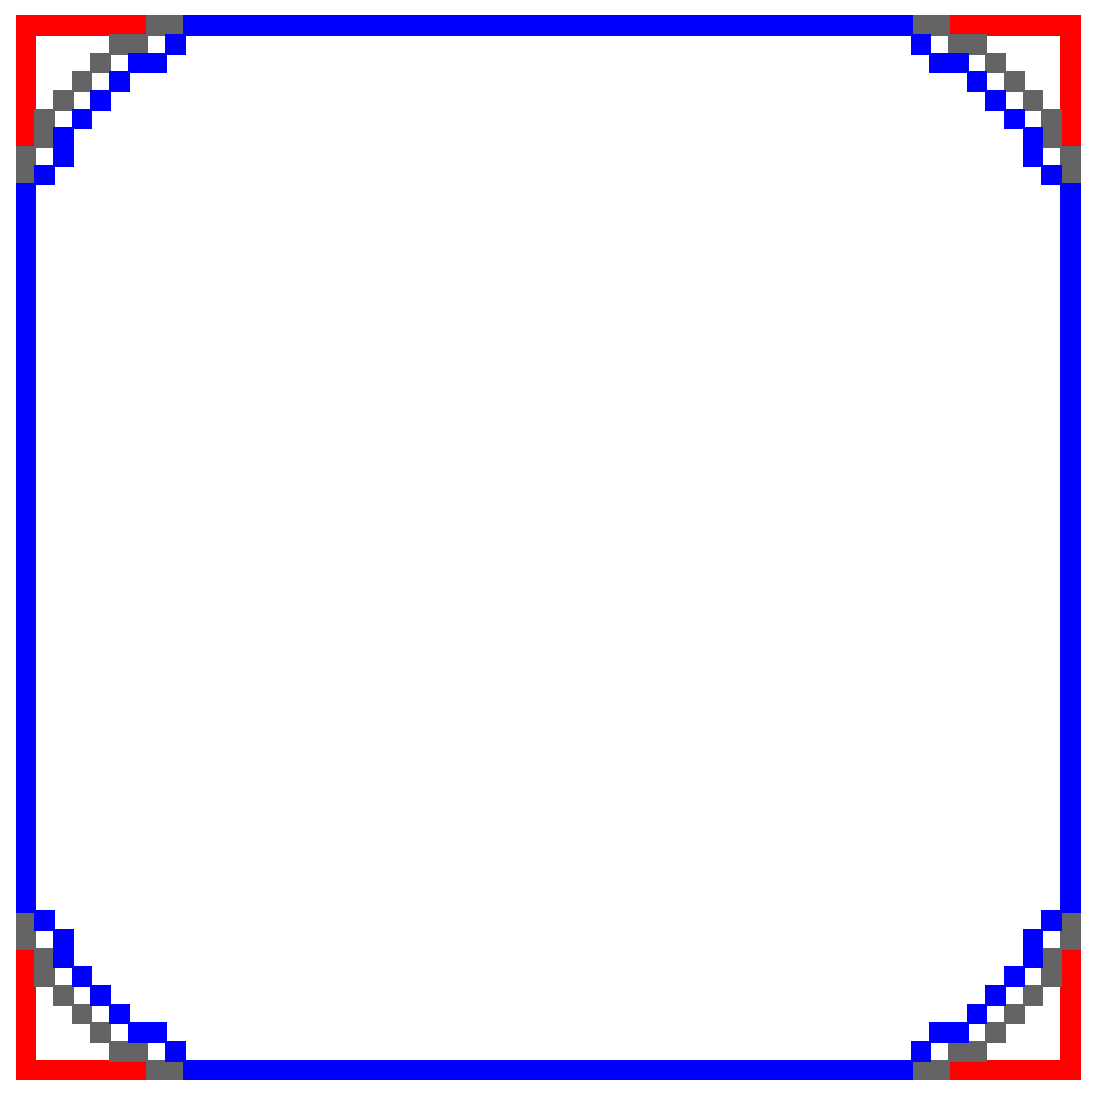
\includegraphics[scale=0.15]{images/flow/grid-radius-effect/square/r3-h0.5/summary_flow.eps}}%
		\hspace{15pt}
		\subfloat{%
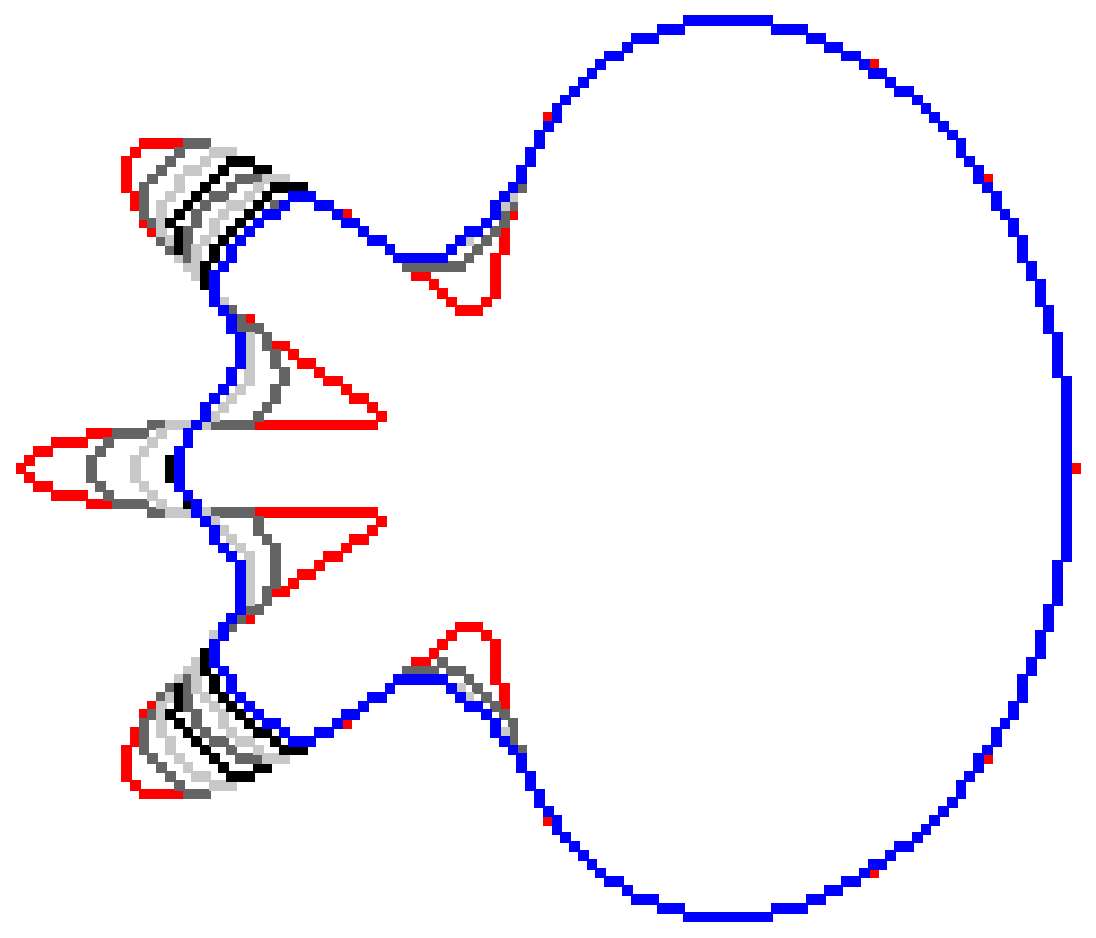
\includegraphics[scale=0.2]{images/flow/grid-radius-effect/flower/r3-h0.5/summary_flow.eps}}%
		}		
	
		\setcounter{subfigure}{-2}
		\subfloat[$r=5,h=0.5$]{%
		\subfloat{%
		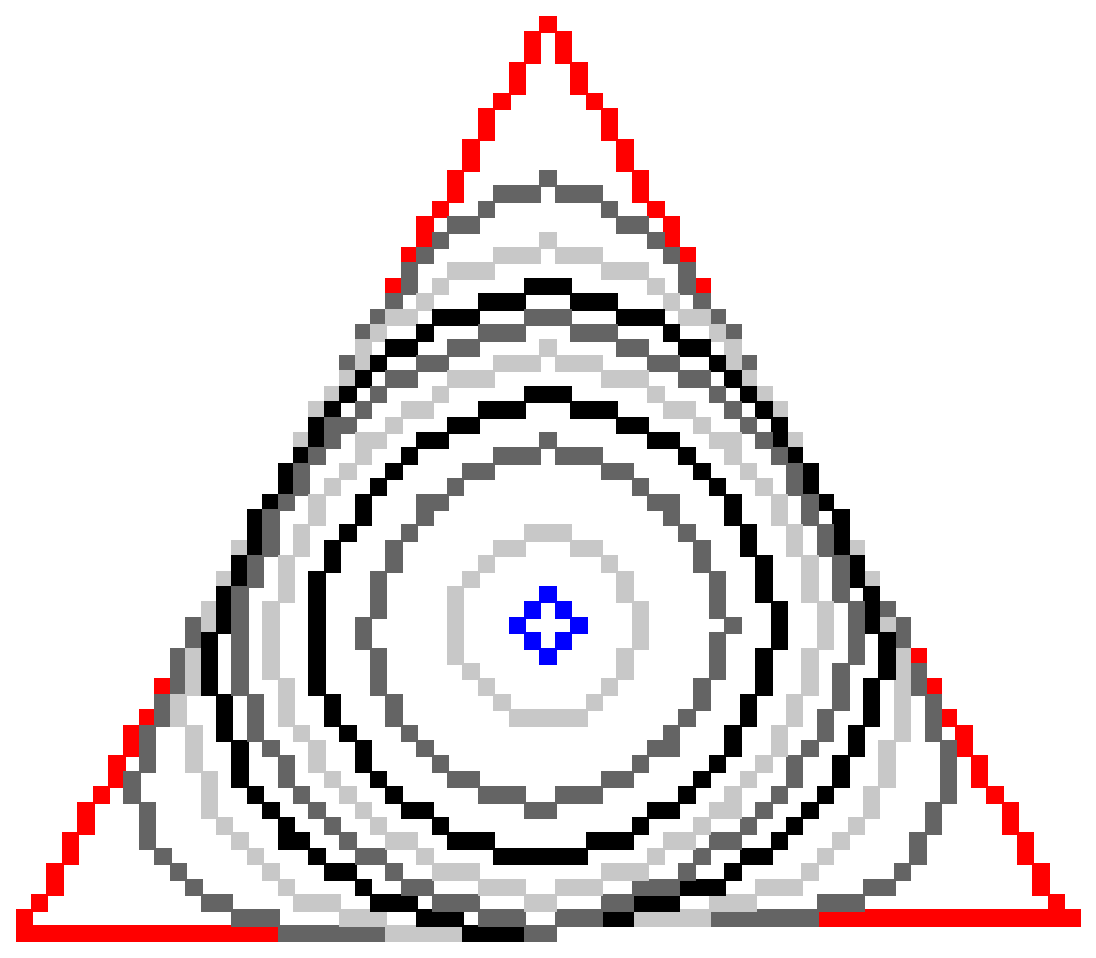
\includegraphics[scale=0.2]{images/flow/grid-radius-effect/triangle/r5-h0.5/summary_flow.eps}
		}%1
		\hspace{15pt}
		\subfloat{%
		\includegraphics[scale=0.15]{images/flow/grid-radius-effect/square/r5-h0.5/summary_flow.eps}}%
		\hspace{15pt}
		\subfloat{%
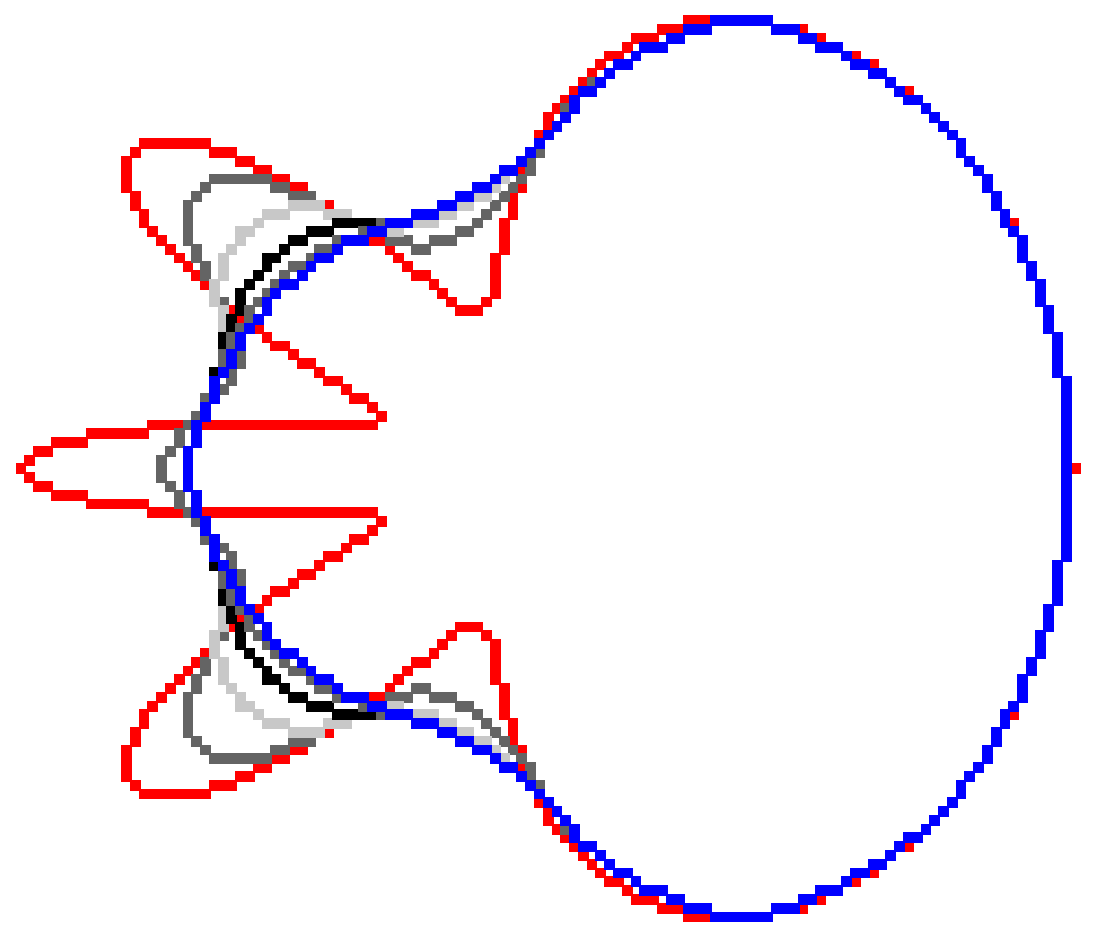
\includegraphics[scale=0.2]{images/flow/grid-radius-effect/flower/r5-h0.5/summary_flow.eps}}%
		}\\
		\subfloat[\revision{Digital elastica evaluation ($r=5,h=0.5$)}]{%
		\includegraphics[scale=0.5]{images/flow/elastica-energy-plot/square-flower-triangle.eps}						
		}
\caption{The choice of radius impacts the flow. In the figures, the flow ceases to evolve for all shapes  when $r=3$ (a). In figure (b), for $r=5$, the triangle evolves to a single point, while the others stop  in an intermediate shape, as in (a). In figure (c), we observe that for a given choice of radius, the digital elastica may increase after a certain number of iterations. }
\label{fig:mx-flow-gs-radius-effect}
\end{figure}


\begin{figure}[!h]
\center
\subfloat[]{%
	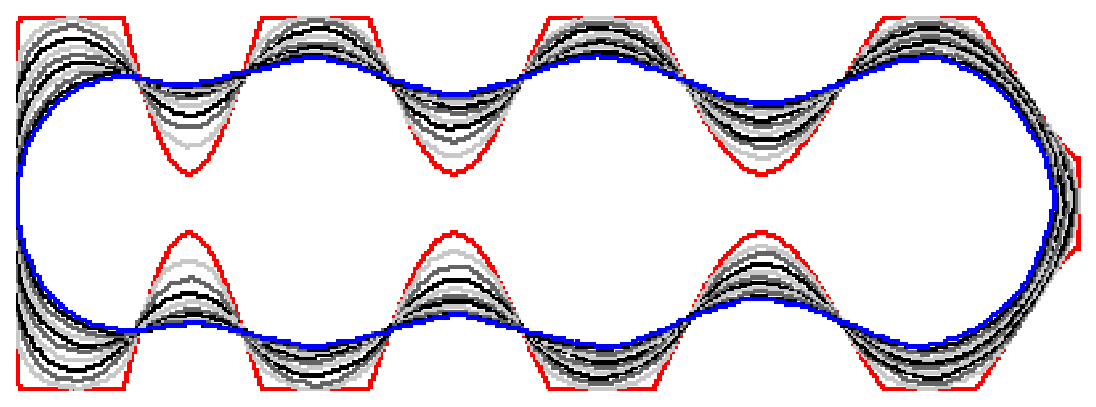
\includegraphics[scale=0.5]{images/flow/faster-high-curvature/summary_flow.eps}}\\%
\subfloat[]{%
		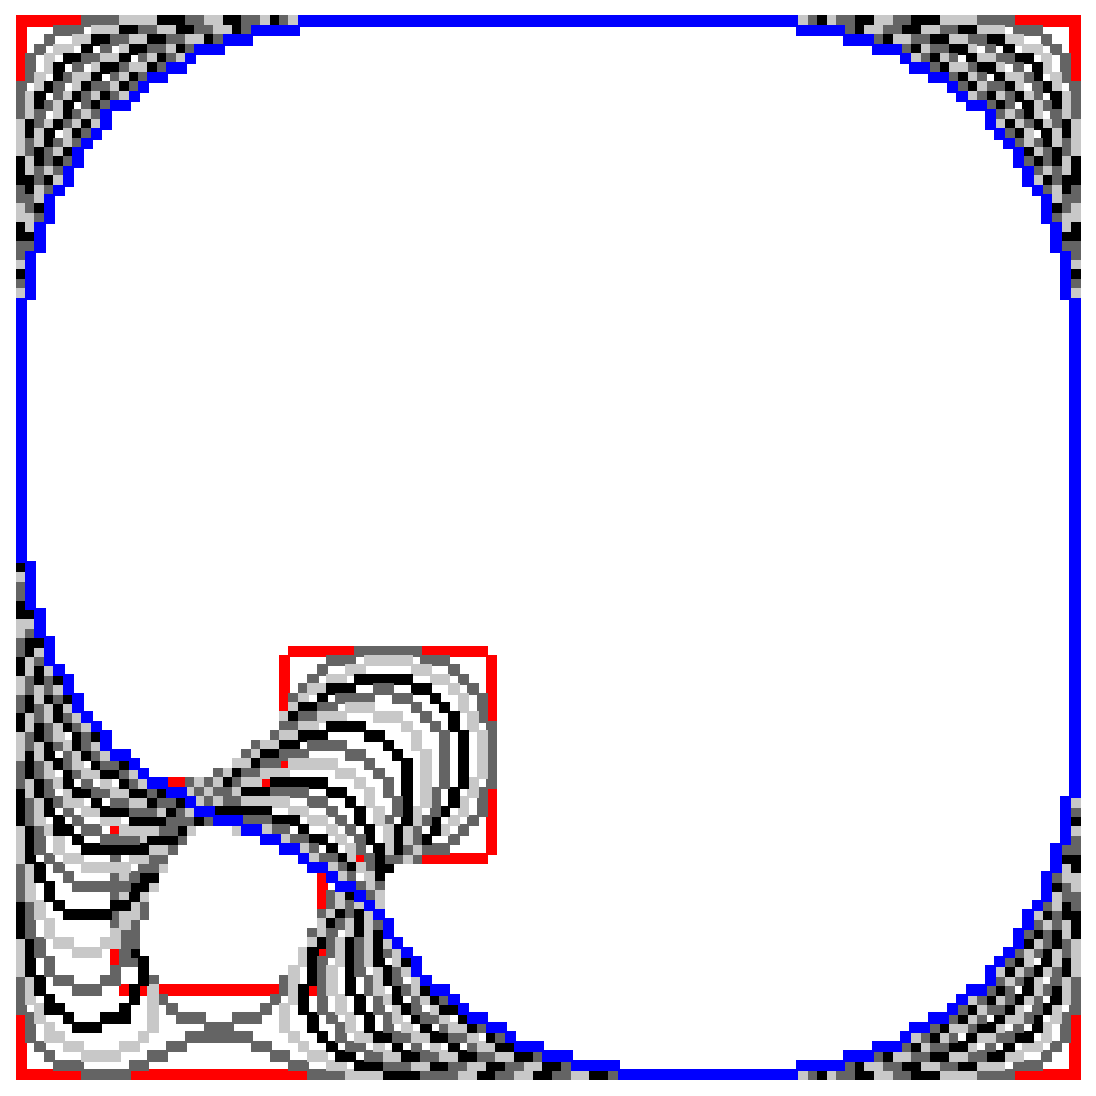
\includegraphics[scale=0.25]{images/flow/fill-holes/summary_flow.eps}}%%1
\caption{High curvature regions evolves faster than lower ones (a). The flow can handle topological changes (b). }
\label{fig:mx-speed-variation-hole-filling}
\end{figure}


\subsection{Optimization method}

Let $f$ be a function of $n$ binary variables with unary and pairwise terms, i.e.

\begin{align*}
f(y_1,\cdots, y_n) = \sum_{j}{f_j(y_j)} + \sum_{j < k}{f_{j,k}(y_j,y_k)}.
\end{align*}

The function $f$ is submodular if and only if the following inequality holds for each pairwise term $f_{j,k}$ \cite{kolmogorov04whatenergies}:
\begin{align*}
  \quad f_{j,k}(0,0) + f_{j,k}(1,1) \leq f_{j,k}(0,1) + f_{j,k}(1,0).
\end{align*}

The energy $E_m$ is non-submodular and optimizing it is a difficult problem, which constrains us to use heuristics and
approximation algorithms. The QPBO method \cite{rother07qpbo} transforms the original problem in a max-flow/min-cut
formulation and yields a full optimal labeling for submodular energies. For non-submodular energies the method is
guaranteed to return a partial labeling with the property that the set of labeled variables is part of an optimal
solution. That property is called partial optimality.

In practice, QPBO can leave many pixels unlabeled. There exist two extensions to QPBO that alleviate this limitation:
QPBOI (improve) and QPBOP (probe). The first is an approximation method that is guaranteed to not increase the energy,
but loses the property of partial optimality. The second is an exact method which is reported to label more variables
than QPBO.

The percentage of unlabeled pixels by QPBOP for $E_1$ is quite high, but the percentage decreases to zero as we set $m$
equal to $r$. Therefore, we are more confident in taking the solution for values of $m$ close to $r$. However, the way it
varies across values of $m$ differs from shape to shape, as is illustrated in figure
\ref{fig:unlabeled-versus-iterations}. We also noticed that, for $m=r$, all the pixels were labeled, {which may
  indicate that $E_r$ is an easy instance of the general non-submodular energy $E_m$, but this remains to be
  proved. The number of pairwise terms in $E_r$ is roughly half of those in $E_1$ (see figure
  \ref{fig:ratio-pairwise-terms}).

  We have used QPBOI to solve $E_m$. Naturally, in the case where all pixels are labeled by QPBOP, QPBOI returns the
  same labeling as QPBOP.


\begin{figure}
\center
\includegraphics[scale=0.5]{images/optimization/pairwise-ratio/plot-pairwiseratio-lowerHigher-concavities-probe.eps}
\caption{We plot the ratio of pairwise terms among all $\binom{|X^{(i)}|}{2}$ combinations. The highest ring has roughly half the number of pairwise terms as the lowest ring.}
\label{fig:ratio-pairwise-terms}
\end{figure}


\begin{figure}[]
\center
\begin{minipage}[b]{0.5\textwidth}
\subfloat[]{ \includegraphics[scale=0.35]{images/optimization/unlabeled-iterations/radius-3/plot-model-square-concavities-probe.eps}}\\%
\subfloat[]{ \includegraphics[scale=0.35]{images/optimization/unlabeled-iterations/radius-5/plot-model-square-concavities-probe.eps}}\\%
\subfloat[]{ \includegraphics[scale=0.35]{images/optimization/unlabeled-iterations/radius-7/plot-model-square-concavities-probe.eps}}%
\end{minipage}%
\begin{minipage}[b]{0.5\textwidth}
\subfloat[]{ \includegraphics[scale=0.35]{images/optimization/unlabeled-iterations/radius-3/plot-model-flower-concavities-probe.eps}}\\%
\subfloat[]{ \includegraphics[scale=0.35]{images/optimization/unlabeled-iterations/radius-5/plot-model-flower-concavities-probe.eps}}\\%
\subfloat[]{ \includegraphics[scale=0.35]{images/optimization/unlabeled-iterations/radius-7/plot-model-flower-concavities-probe.eps}}%
\end{minipage}
\caption{For each plot, we first produce shapes $\left\{ S^{(i)} \right\}$ executing DCE with $m=r$. Then, for each shape in $\left\{ S^{(i)} \right\}$, we execute one iteration of DCE for different values of $m$ and we count the unlabeled pixels. The number of unlabeled pixels by QPBOP remains high for lower values of $m$, and goes to zero when $m=r$. We observe the same behaviour for varying radius values.}
\label{fig:unlabeled-versus-iterations}
\end{figure}

\section{Application to image segmentation}

We present an application of our digital curve evolution algorithm to supervised image segmentation. The DCE acts as a
contour correction method. Here we use a data fidelity term in order to characterize the object of
interest. Given foreground and background seeds selected by the user, we derive mixed Gaussian distributions of color
intensities $G_f$,$G_b$, and we define the data fidelity term as the cross-entropy, i.e.
	
\begin{align}
  g(y) = -(1-y)\log{G_f(I(y))} - y\log{G_b(I(y))}.
  \label{eq:data-fidelity}
\end{align}	

We use the DCE algorithm to regularize an initial contour output by some segmentation algorithm or delineated by the user. In this application, the \revision{data} term of the DCE
is set to the data fidelity term \eqref{eq:data-fidelity}.
	
\begin{algorithm}
 \SetKwData{It}{i}
 \SetKwData{MIt}{maxIt}
 \SetKwData{Tol}{tolerance}
 \SetKwData{Delta}{delta}
 \SetKwInOut{Input}{input}\SetKwInOut{Output}{output}
 \SetKwComment{comment}{//}{}
 
 \Input{An image $I$; seed mask $M$; the estimation ball radius $r$; length $(\alpha)$, squared curvature $(\beta)$ and data fidelity $(\gamma)$ coefficients; initial dilation $d$; stop condition value \Tol; the maximum number of iterations \MIt;}
 \BlankLine

 $S \longleftarrow$ GrabCut($I,M$)\;
 $S^{(0)} \longleftarrow $ dilate($S$,$d$)\; 
 \Delta $\longleftarrow +\infty$\;
 $i \longleftarrow 0$\;
 \While{ \It $<$ \MIt \bf{and} \Delta $>$ \Tol  }{ 	
 	$S^{(i+1)} \longleftarrow $ DCE($S^{(i)},r,\alpha,\beta,\gamma,2$)\;
 	\Delta $\longleftarrow |S^{(i)} - S^{(i+1)}|$\;

	\It $\longleftarrow$ \It $+1$\;
	
 }
 \label{alg:contour-correction} 
 \caption{Contour correction algorithm.}
\end{algorithm}	

The algorithm can be initialized by a collection of compact sets, or with the result of a third-party segmentation algorithm, as GrabCut \cite{rother04grabcut}. We include an additional parameter $d$ that dilates the initial sets using a square of side one before executing the flow.
	
\begin{figure}[ht!]
\center
\begin{tabular}{ccc}
\revision{Seeds} & $(\alpha=0, \beta=0.5)$ & $(\alpha=0,\beta=1)$ \\
 	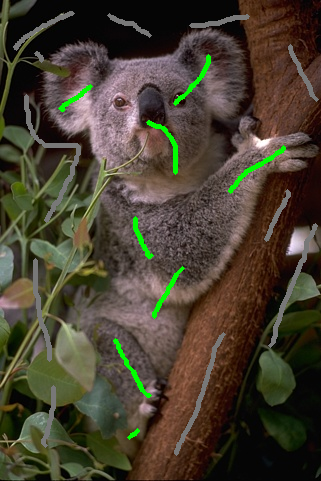
\includegraphics[scale=0.25]{images/segmentation/bc/coala/seeds.png} & 
	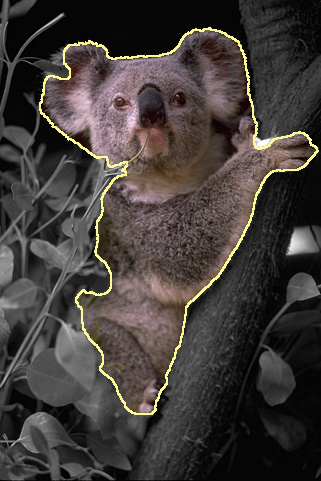
\includegraphics[scale=0.25]{images/segmentation/bc/coala/r3/lg0_sq05_dt1_it50.png} & 
	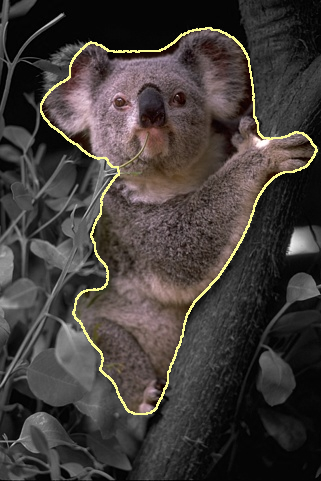
\includegraphics[scale=0.25]{images/segmentation/bc/coala/r3/lg0_sq1_dt1_it50.png} \\
	
 	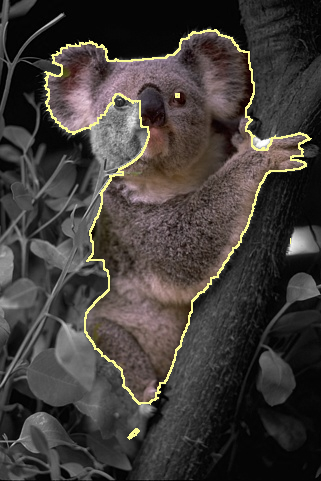
\includegraphics[scale=0.25]{images/segmentation/bc/coala/grabcut-seg.png} & 
	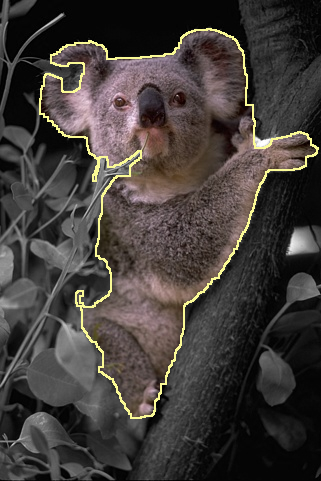
\includegraphics[scale=0.25]{images/segmentation/bc/coala/r3/lg1_sq0_dt1_it50.png} &
	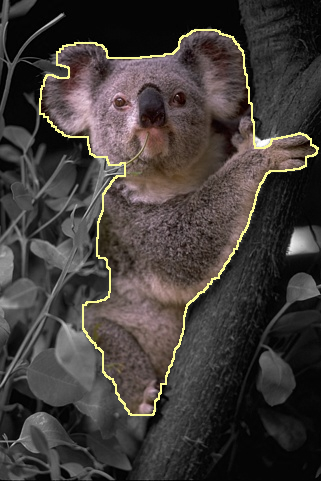
\includegraphics[scale=0.25]{images/segmentation/bc/coala/r3/lg2_sq0_dt1_it50.png} \\

	\revision{GrabCut} & $(\alpha=0.5, \beta=0)$ & $(\alpha=1, \beta=0)$
\end{tabular}	
\caption{Comparison of squared curvature regularization (first row) and length regularization (second row). }
\label{fig:parameters-influence}
\end{figure}

\begin{figure}[ht!]
	\center
	\begin{tabular}{ccc}
		GrabCut & Schoenemann & Contour Correction \\
		& $(\alpha=0.1, \beta=1.0$) & $(r=5, \alpha=0.1, \beta=1.0, \gamma=3.0$)\\
		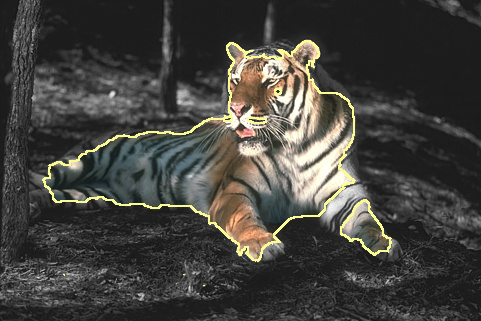
\includegraphics[scale=0.2]{images/segmentation/bc/tiger1/gc-seg.png} &
	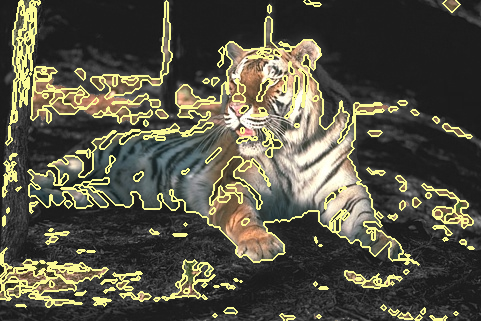
\includegraphics[scale=0.2]{images/segmentation/schoenemann/tiger1/tiger1-seg.png}&
		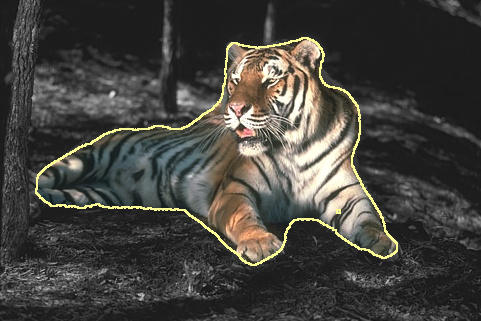
\includegraphics[scale=0.2]{images/segmentation/bc/tiger1/corrected-seg.png}\\									
		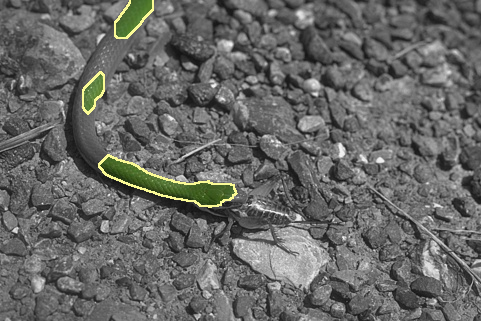
\includegraphics[scale=0.2]{images/segmentation/bc/snake/gc-seg.png} &
		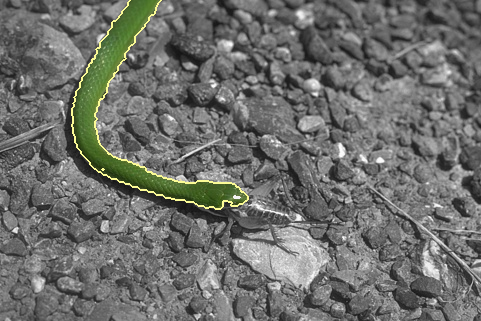
\includegraphics[scale=0.2]{images/segmentation/schoenemann/snake/snake-seg.png} &
		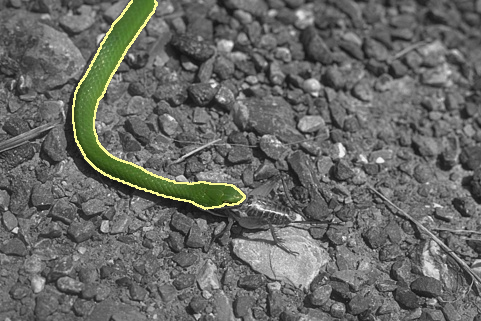
\includegraphics[scale=0.2]{images/segmentation/bc/snake/corrected-seg.png}\\
		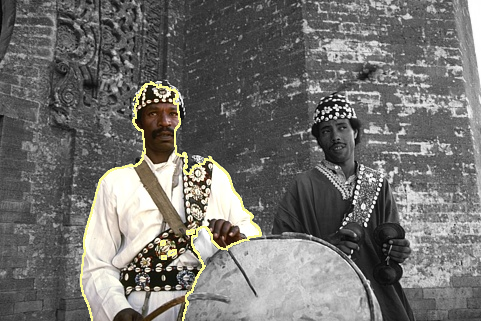
\includegraphics[scale=0.2]{images/segmentation/bc/man/gc-seg.png} &
		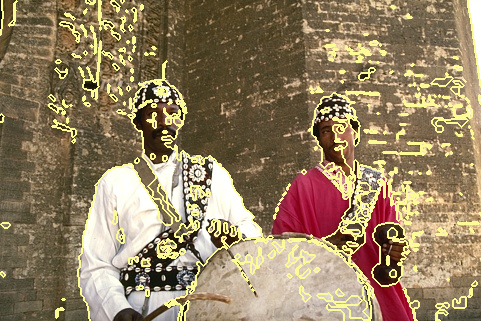
\includegraphics[scale=0.2]{images/segmentation/schoenemann/man/man-seg.png} &
		\includegraphics[scale=0.2]{images/segmentation/bc/man/corrected-seg.png}\\		
		\includegraphics[scale=0.2]{images/segmentation/bc/vase/gc-seg.png} &
		\includegraphics[scale=0.2]{images/segmentation/schoenemann/vase/vase-seg.png} &
		\includegraphics[scale=0.2]{images/segmentation/bc/vase/corrected-seg.png}		
	\end{tabular}
	\caption{The proposed method regularizes GrabCut \cite{rother04grabcut} contours and returns meaningful results. We can observe the completion feature of curvature in the second row, and we don't suffer from over-segmentation issues as Schoenemann's method \cite{schoenemann09linear}. However, our flow may stop in a local optimum as in the fourth row, while Schoenemann's is able to extrapolate such solutions.}
	\label{fig:segmentation-results}	
\end{figure}


\begin{figure}[hp!]
	\center
	\begin{tabular}{ccc}
		GrabCut & Schoenemann & Contour Correction \\
		& $(\alpha=0.1, \beta=1.0$) & $(r=5, \alpha=0.1, \beta=1.0, \gamma=3.0$)\\
		\includegraphics[scale=0.2]{images/segmentation/bc/airplane2/gc-seg.png} &
		\includegraphics[scale=0.2]{images/segmentation/schoenemann/airplane2/airplane2-seg.png} &
		\includegraphics[scale=0.2]{images/segmentation/bc/airplane2/corrected-seg.png}\\						
		\includegraphics[scale=0.2]{images/segmentation/bc/bird/gc-seg.png} &
		\includegraphics[scale=0.2]{images/segmentation/schoenemann/bird/bird-seg.png} &
		\includegraphics[scale=0.2]{images/segmentation/bc/bird/corrected-seg.png}\\				
		\includegraphics[scale=0.2]{images/segmentation/bc/camel/gc-seg.png} &
		\includegraphics[scale=0.2]{images/segmentation/schoenemann/camel/camel-seg.png} &
		\includegraphics[scale=0.2]{images/segmentation/bc/camel/corrected-seg.png}\\	
		\includegraphics[scale=0.2]{images/segmentation/bc/rock/gc-seg.png} &
		\includegraphics[scale=0.2]{images/segmentation/schoenemann/rock/rock-seg.png} &
		\includegraphics[scale=0.2]{images/segmentation/bc/rock/corrected-seg.png} \\		
		\includegraphics[scale=0.2]{images/segmentation/bc/giraffes/gc-seg.png} &
		\includegraphics[scale=0.2]{images/segmentation/schoenemann/giraffes/giraffes-seg.png} &
		\includegraphics[scale=0.2]{images/segmentation/bc/giraffes/corrected-seg.png} \\		
		\includegraphics[scale=0.2]{images/segmentation/bc/canguru/gc-seg.png} &
		\includegraphics[scale=0.2]{images/segmentation/schoenemann/canguru/canguru-seg.png} &
		\includegraphics[scale=0.2]{images/segmentation/bc/canguru/corrected-seg.png} \\		
		\includegraphics[scale=0.2]{images/segmentation/bc/coral/gc-seg.png} &
		\includegraphics[scale=0.2]{images/segmentation/schoenemann/coral/coral-seg.png} &
		\includegraphics[scale=0.2]{images/segmentation/bc/coral/corrected-seg.png}								
	\end{tabular}
	\caption{\revision{Additional comparison results between GrabCut \cite{rother04grabcut}, Schoenemman  \cite{schoenemann09linear} and Contour correction segmentation methods.}}
	\label{fig:more-segmentation-results}	
\end{figure}


We evaluate our method using the BSD300 database \cite{martinFTM01berkeley}. All images contain the same number of pixels, \revision{the resolution being 321x481 (481x321) in portrait (landscape) mode}. We compare the results of our method with segmentations given by GrabCut and Schoenemanns's method \cite{schoenemann09linear}. We report an average of $3s$ per flow iteration, and an average of $30$ iterations per image. While GrabCut executes in less than one second, Schoenemann's method may take several hours to complete.


{In figure \ref{fig:parameters-influence} we can observe the results of a curvature regularization in comparison with a
  pure length regularization. The curvature can fill gaps and is smoother than the one produced by length only,
  resulting in more pleasant segmentations. In figures \ref{fig:segmentation-results} and
  \ref{fig:more-segmentation-results} we list several results of our method and we compare them with segmentation
  produced by GrabCut and Schoenemann's method. Our method is successful in producing curvature regularized
  segmentations and demonstrates the completion property of curvature. Moreover, it does not suffer from over-segmentation, it is much faster than Schoenemann's, and in several cases produces better segmentations than
  GrabCut.

\section{Conclusion}\label{sec:conclusion}


We have studied in depth several digital curve evolution models based on a digital version of the Elastica energy and we
have presented an application to image segmentation. The processes we have described are completely digital and do not
suffer from issues that typically arise in models that pass through a discretization stage, such as
rounding. Moreover, the model can handle changes in topology and its results are competitive with similar approaches
while achieving reasonable running times.

Future developments of this work will include extending the DCE algorithm to $3$d, as the integral invariant estimator
is available in higher dimensions. As a result, a denoising application may be derived by lifting the flow to $3$d
with a data fidelity defined by image intensities or by distance to initial position.



%
% ---- Bibliography ----
%
% BibTeX users should specify bibliography style 'splncs04'.
% References will then be sorted and formatted in the correct style.
%
\bibliographystyle{splncs04}
\bibliography{jmiv}

\end{document}

